\subsection*{Compressible Flow}

\frame
{
  \frametitle{Compressible Shocked Flow}
  \begin{itemize}[<+->]
    \item Original compressible flow code written by Ben Kirk utilizing libMesh.
      \begin{itemize}[<+->]
      \item Solves both Compressible Navier Stokes and Inviscid Euler.
      \item Includes both SUPG and a shock capturing scheme.
      \end{itemize}
    \item Original redistribution code written by Larisa Branets.
      \begin{itemize}[<+->]
      \item Simultaneous optimization of element shape and size.
      \item Directable via user supplied error estimate.
      \end{itemize}
    \item Integration work done by Derek Gaston.
      \begin{itemize}[<+->]
      \item Combination of redistribution, $h$ refinement.
      \item Applicable to other problem classes.
      \end{itemize}
  \end{itemize}
}

\frame
{
  \frametitle{Problem Specification}
  \begin{itemize}[<+->]
    \item The problem studied is that of an oblique shock generated by a $10^o$ wedge angle. 
      \begin{itemize}[<+->]
      \item This problem has an exact solution for density which is a step function.
      \item Utilizing libmesh's exact solution capability the exact
$L_2$ error can be solved for.
      \item The exact solution is shown below:
        \begin{figure}
          \begin{center}
            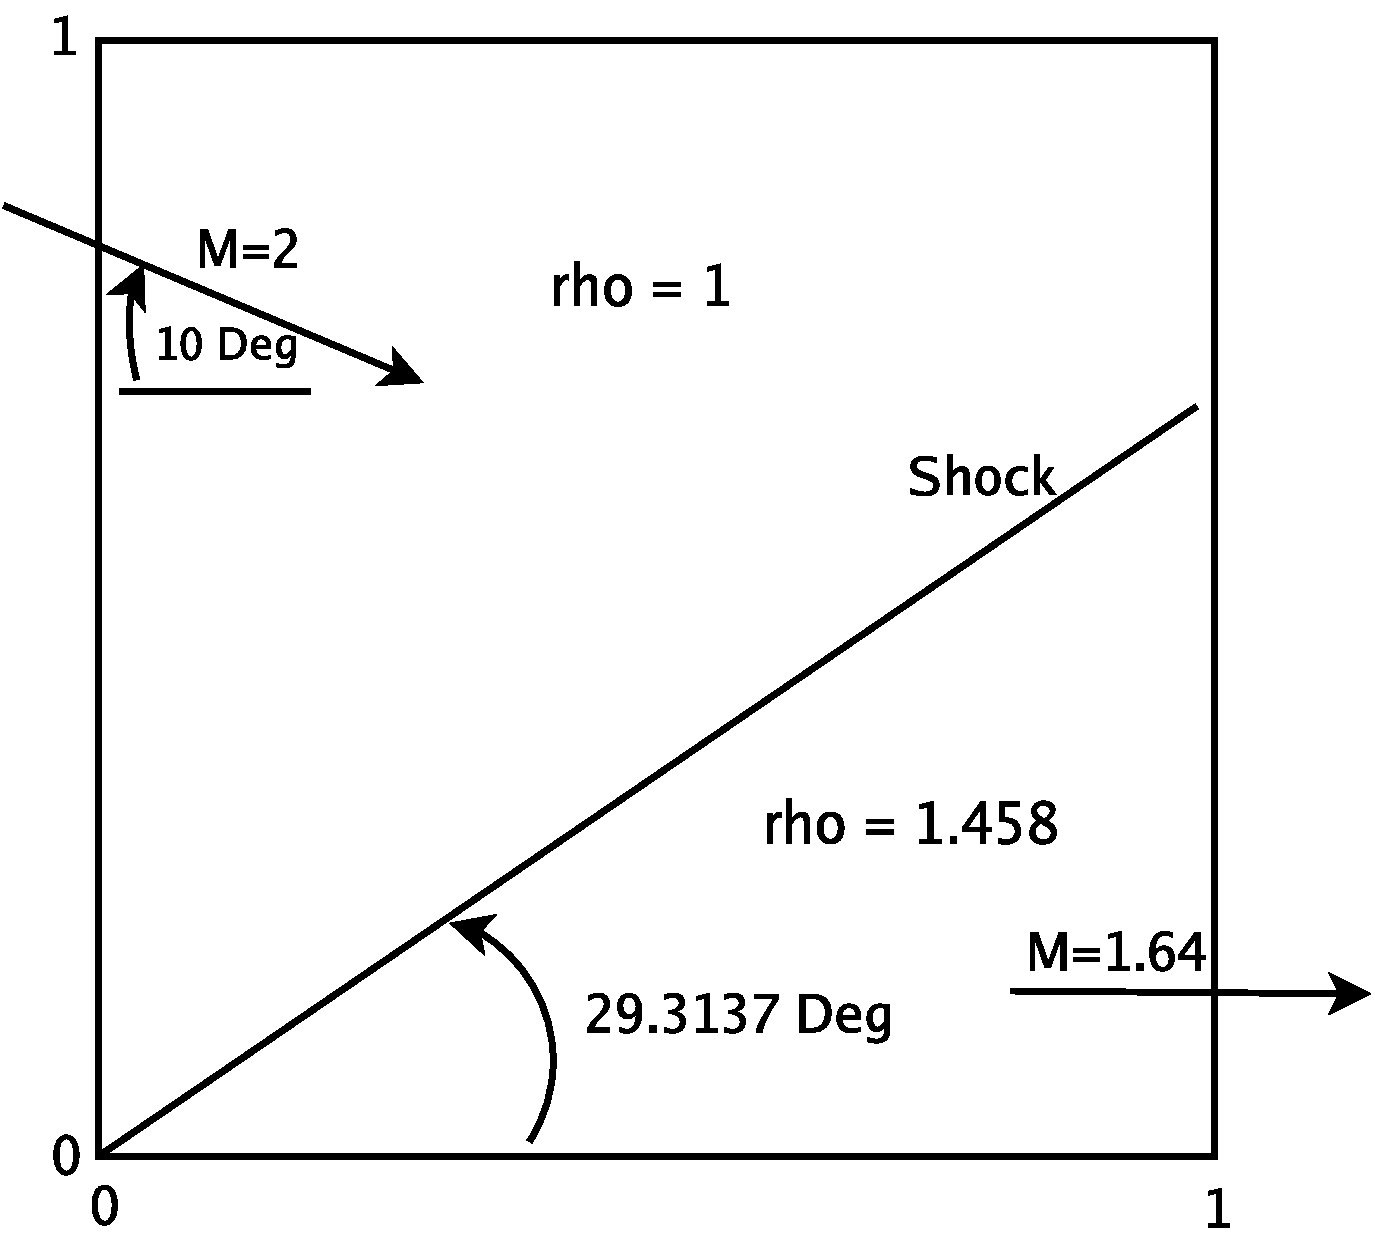
\includegraphics[viewport=20 10 660 600,clip=true,width=.4\textwidth]{shock.pdf}
          \end{center}
        \end{figure}
    \end{itemize}
  \end{itemize}
}

\frame
{
  \frametitle{Uniformly Refined Solutions}
  \begin{itemize}[<+->]
  \item For comparison purposes, here is a mesh and a solution after 1 uniform refinement with 10890 DOFs.
    \begin{figure}[!htb]
      \begin{center}
        \subfigure[Mesh after 1 uniform refinement.]{\label{fig:fob_uniform_2_mesh}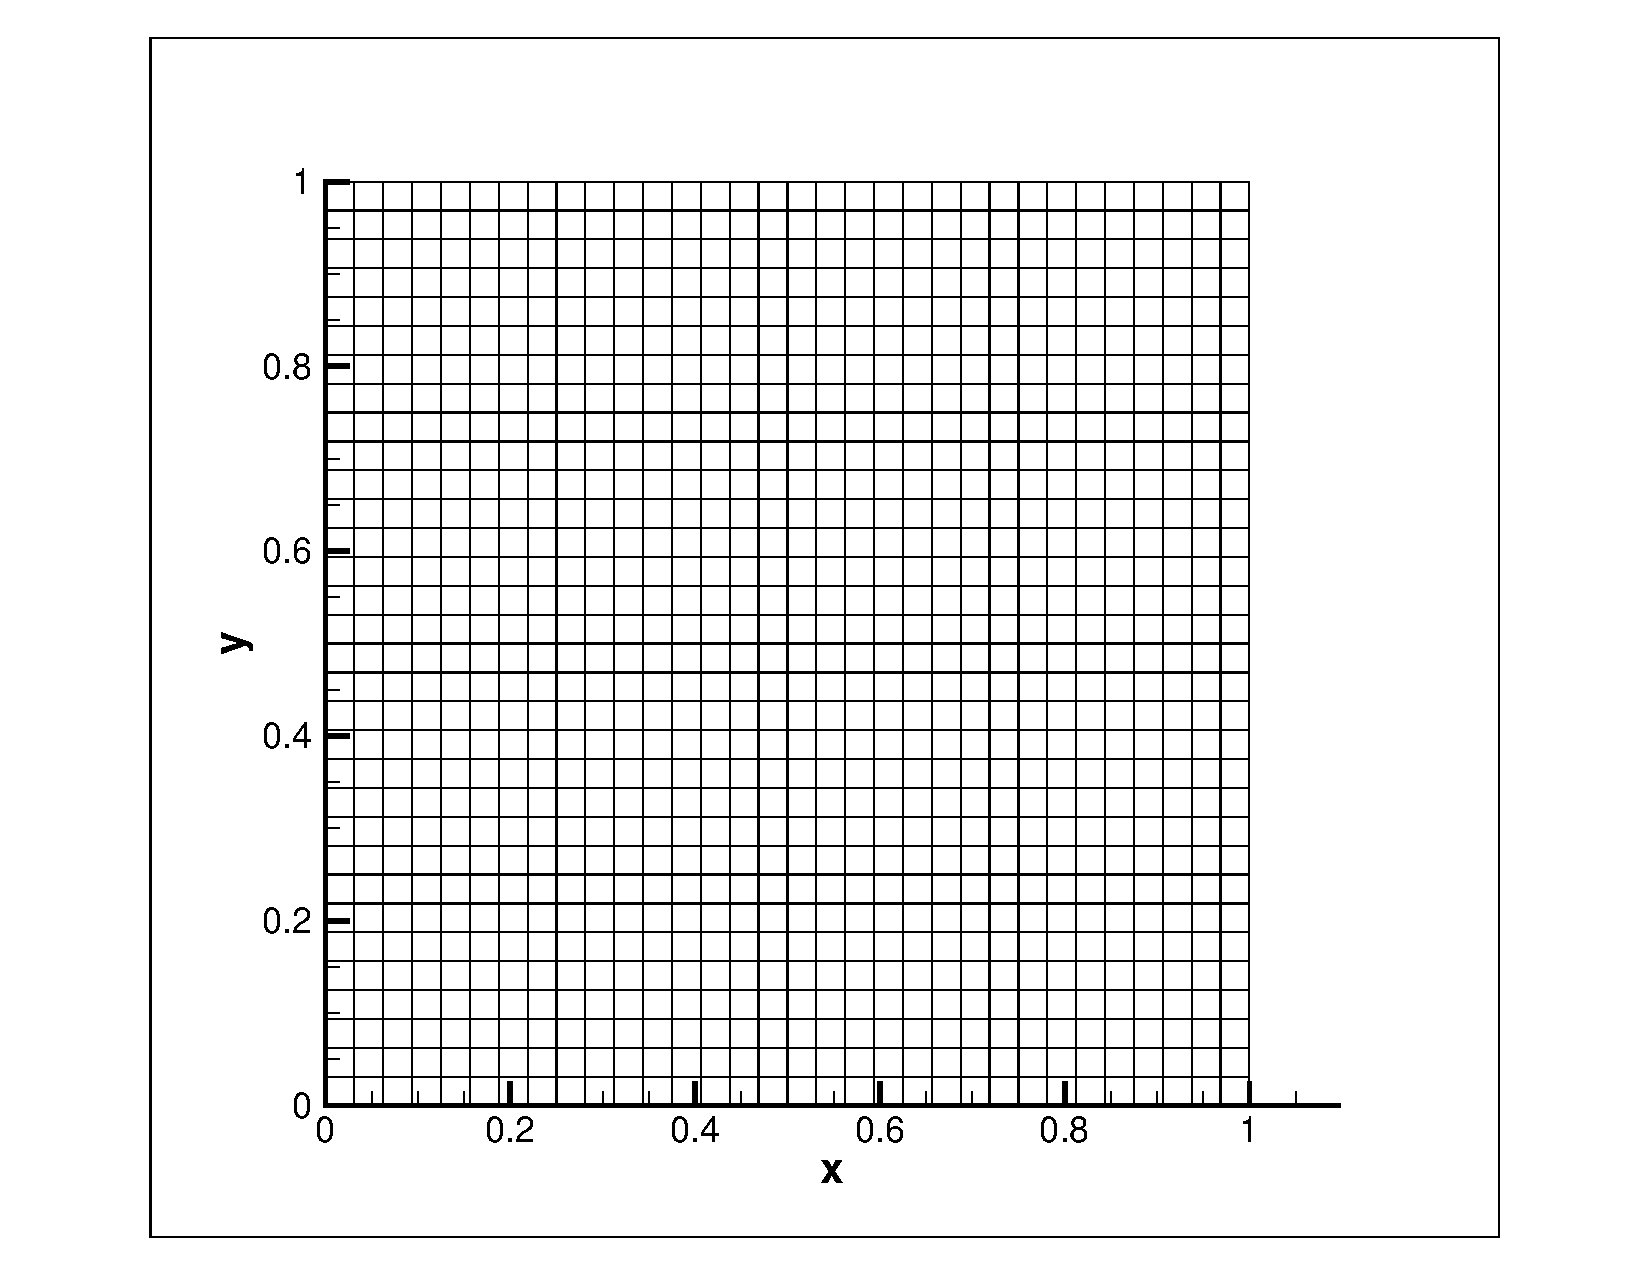
\includegraphics[viewport=110 30 600 550,clip=true,width=.42\textwidth]{fob_uniform_2_mesh.pdf}}
        \subfigure[Solution after 1 uniform refinement.]{\label{fig:fob_uniform_2_sol}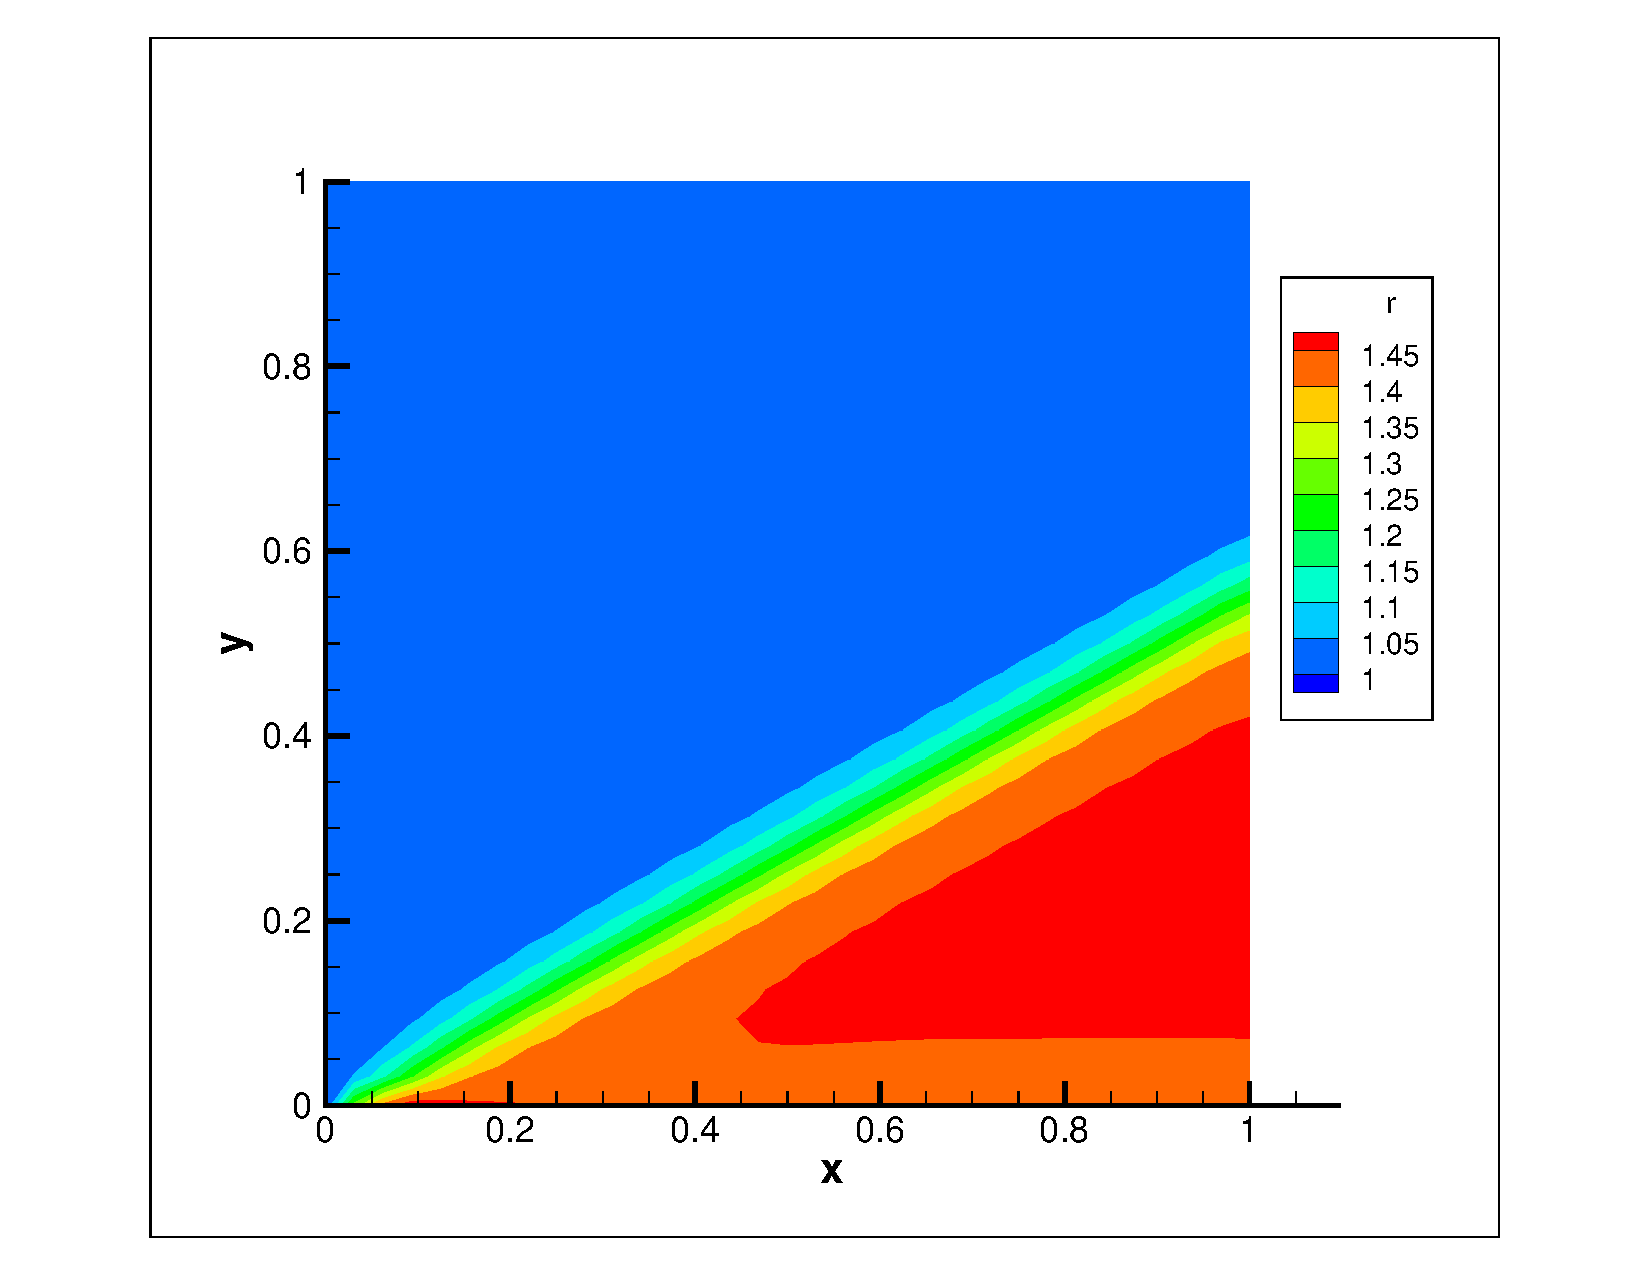
\includegraphics[viewport=110 30 600 520,clip=true,width=.42\textwidth]{fob_uniform_2_sol.pdf}}
      \end{center}
    \end{figure}
  \end{itemize}
}

\frame
{
  \frametitle{H-Adapted Solutions}
  \begin{itemize}[<+->]
    \item A flux jump indicator was employed as the error indcator along with a statistical flagging scheme.
    \item Here is a mesh and solution after 2 adaptive refinements containing 10800 DOFs:
      \begin{figure}[!htb]
        \begin{center}
          \subfigure[Mesh, 2 refinements]{\label{fig:fob_adapt_3_mesh}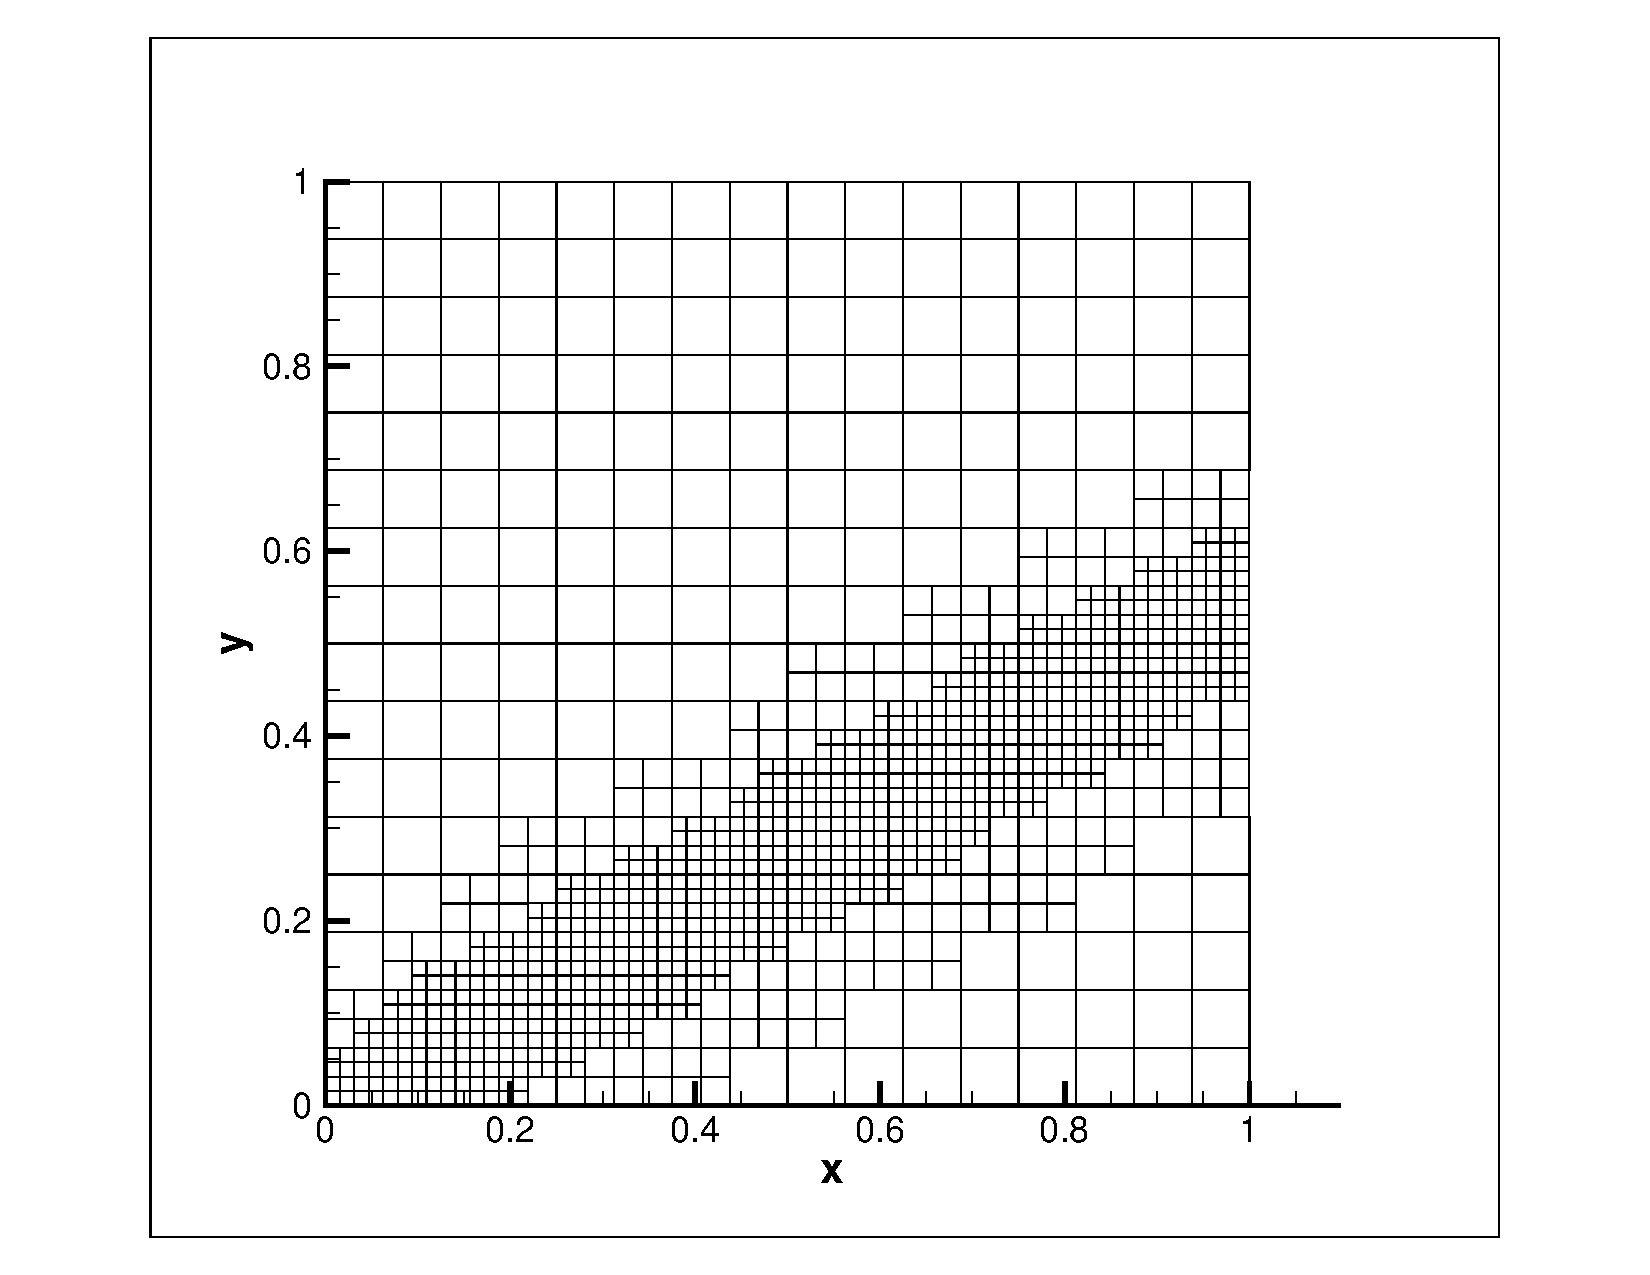
\includegraphics[viewport=110 30 600 550,clip=true,width=.42\textwidth]{fob_adapt_3_mesh.pdf}}
          \subfigure[Solution]{\label{fig:fob_adapt_3_sol}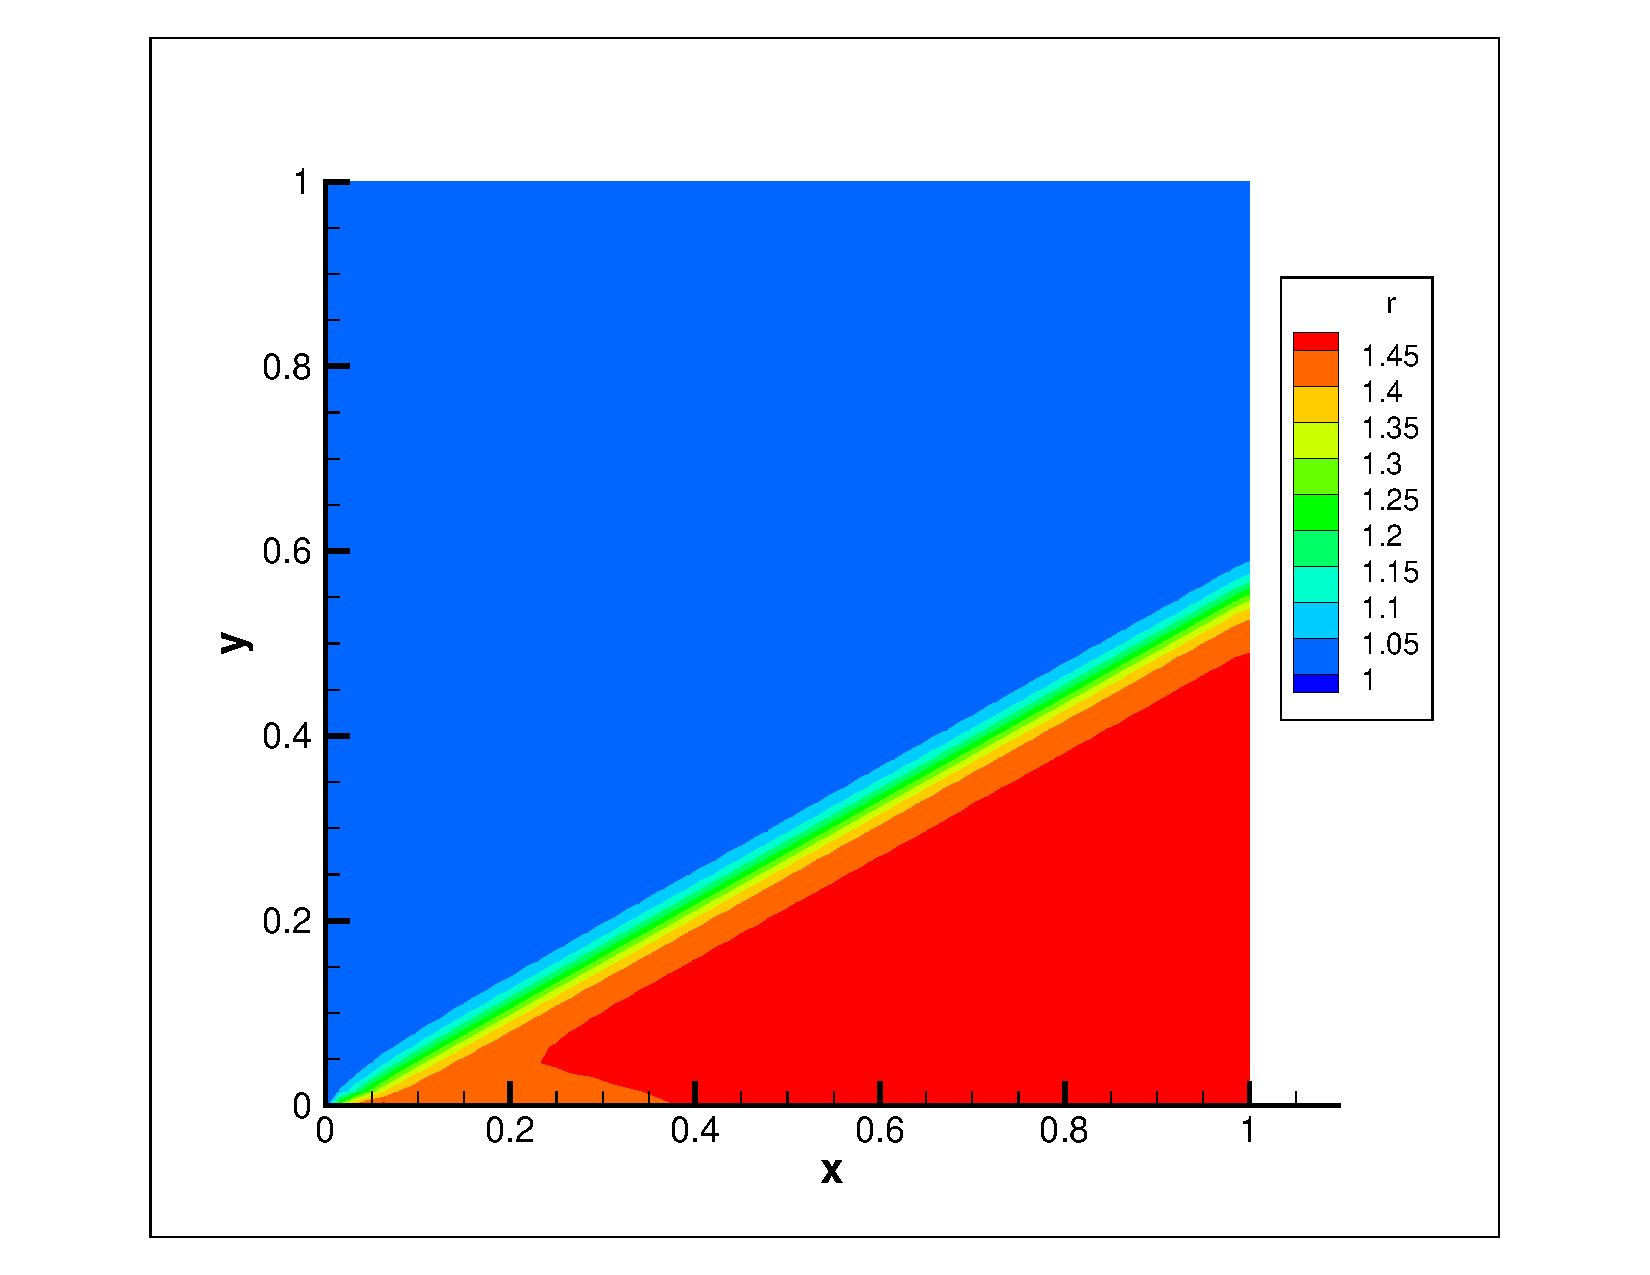
\includegraphics[viewport=110 30 600 520,clip=true,width=.42\textwidth]{fob_adapt_3_sol.pdf}}
        \end{center}
      \end{figure}
  \end{itemize}
}

\frame
{
  \frametitle{Redistributed Solutions}
  \begin{itemize}[<+->]
    \item Redistribution utilizing the same flux jump indicator.
      \begin{figure}[!htb]
        \begin{center}
          \subfigure[Mesh, 8 redistribution steps]{\label{fig:fob_redist_adapt_8_mesh}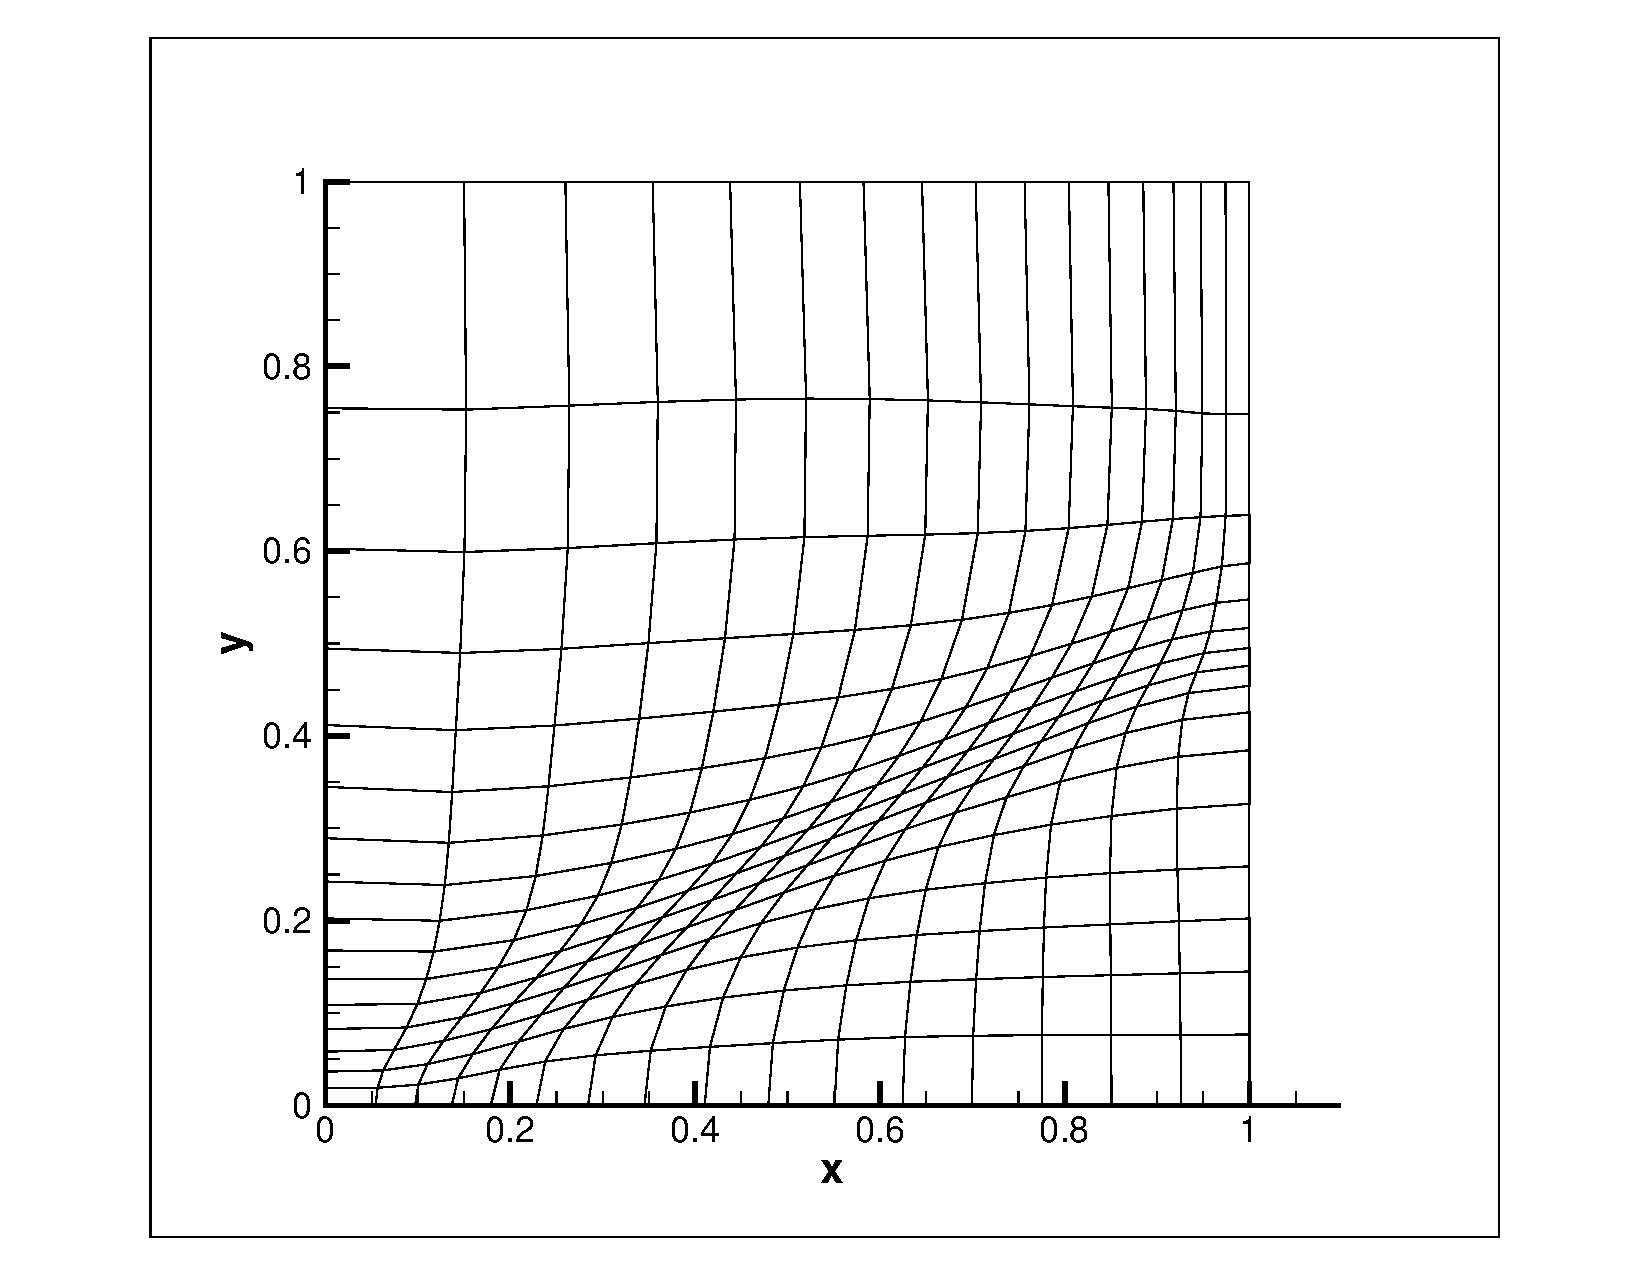
\includegraphics[viewport=110 30 600 550,clip=true,width=.42\textwidth]{fob_redist_adapt_8_mesh.pdf}}
          \subfigure[Solution]{\label{fig:fob_redist_adapt_8_sol}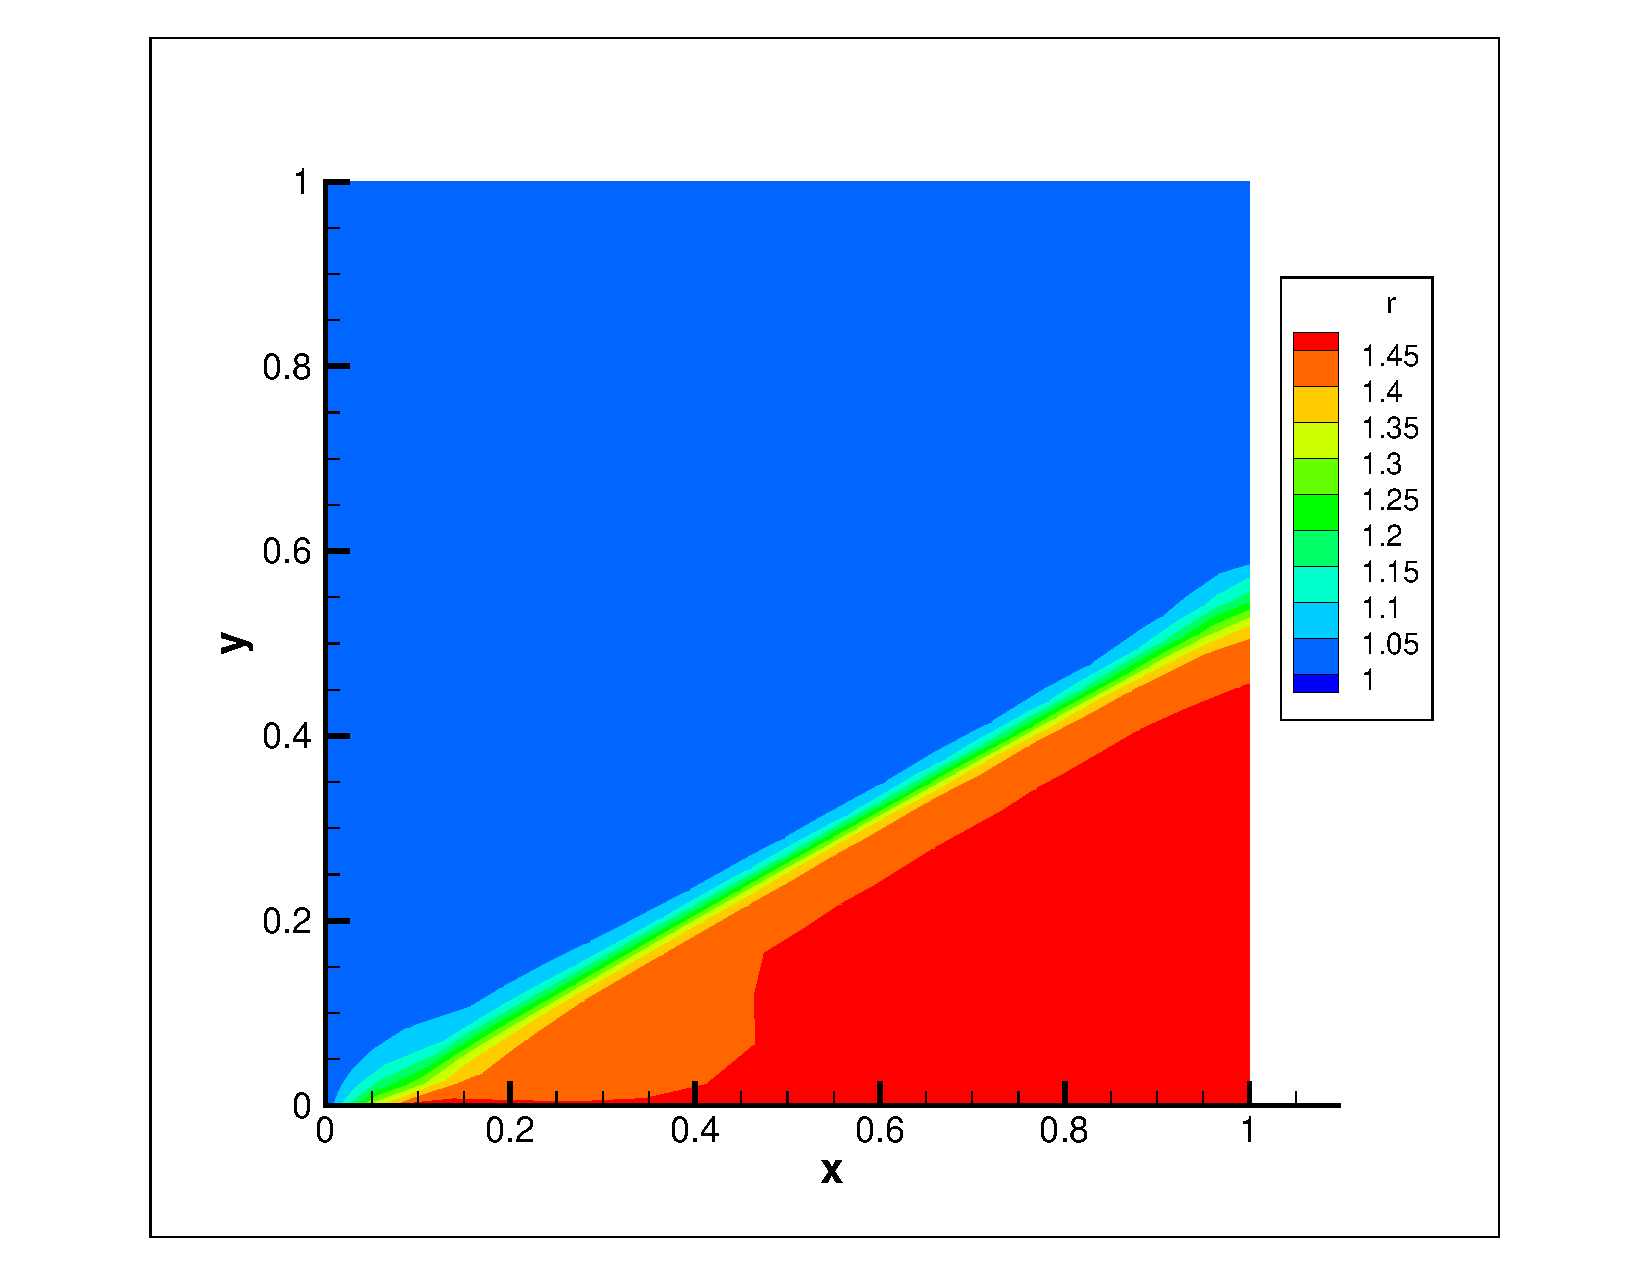
\includegraphics[viewport=110 30 600 520,clip=true,width=.42\textwidth]{fob_redist_adapt_8_sol.pdf}}
        \end{center}
      \end{figure}
  \end{itemize}
}

\frame
{
  \frametitle{Redistributed and Adapted}
  \begin{itemize}[<+->]
    \item Now combining the two, here are the mesh and solution after 2 adaptations beyond the previous redistribution containing 10190 DOFs.
      \begin{figure}[!htb]
        \begin{center}
          \subfigure[Mesh, 2 refinements]{\label{fig:fob_redist_adapt_10_mesh}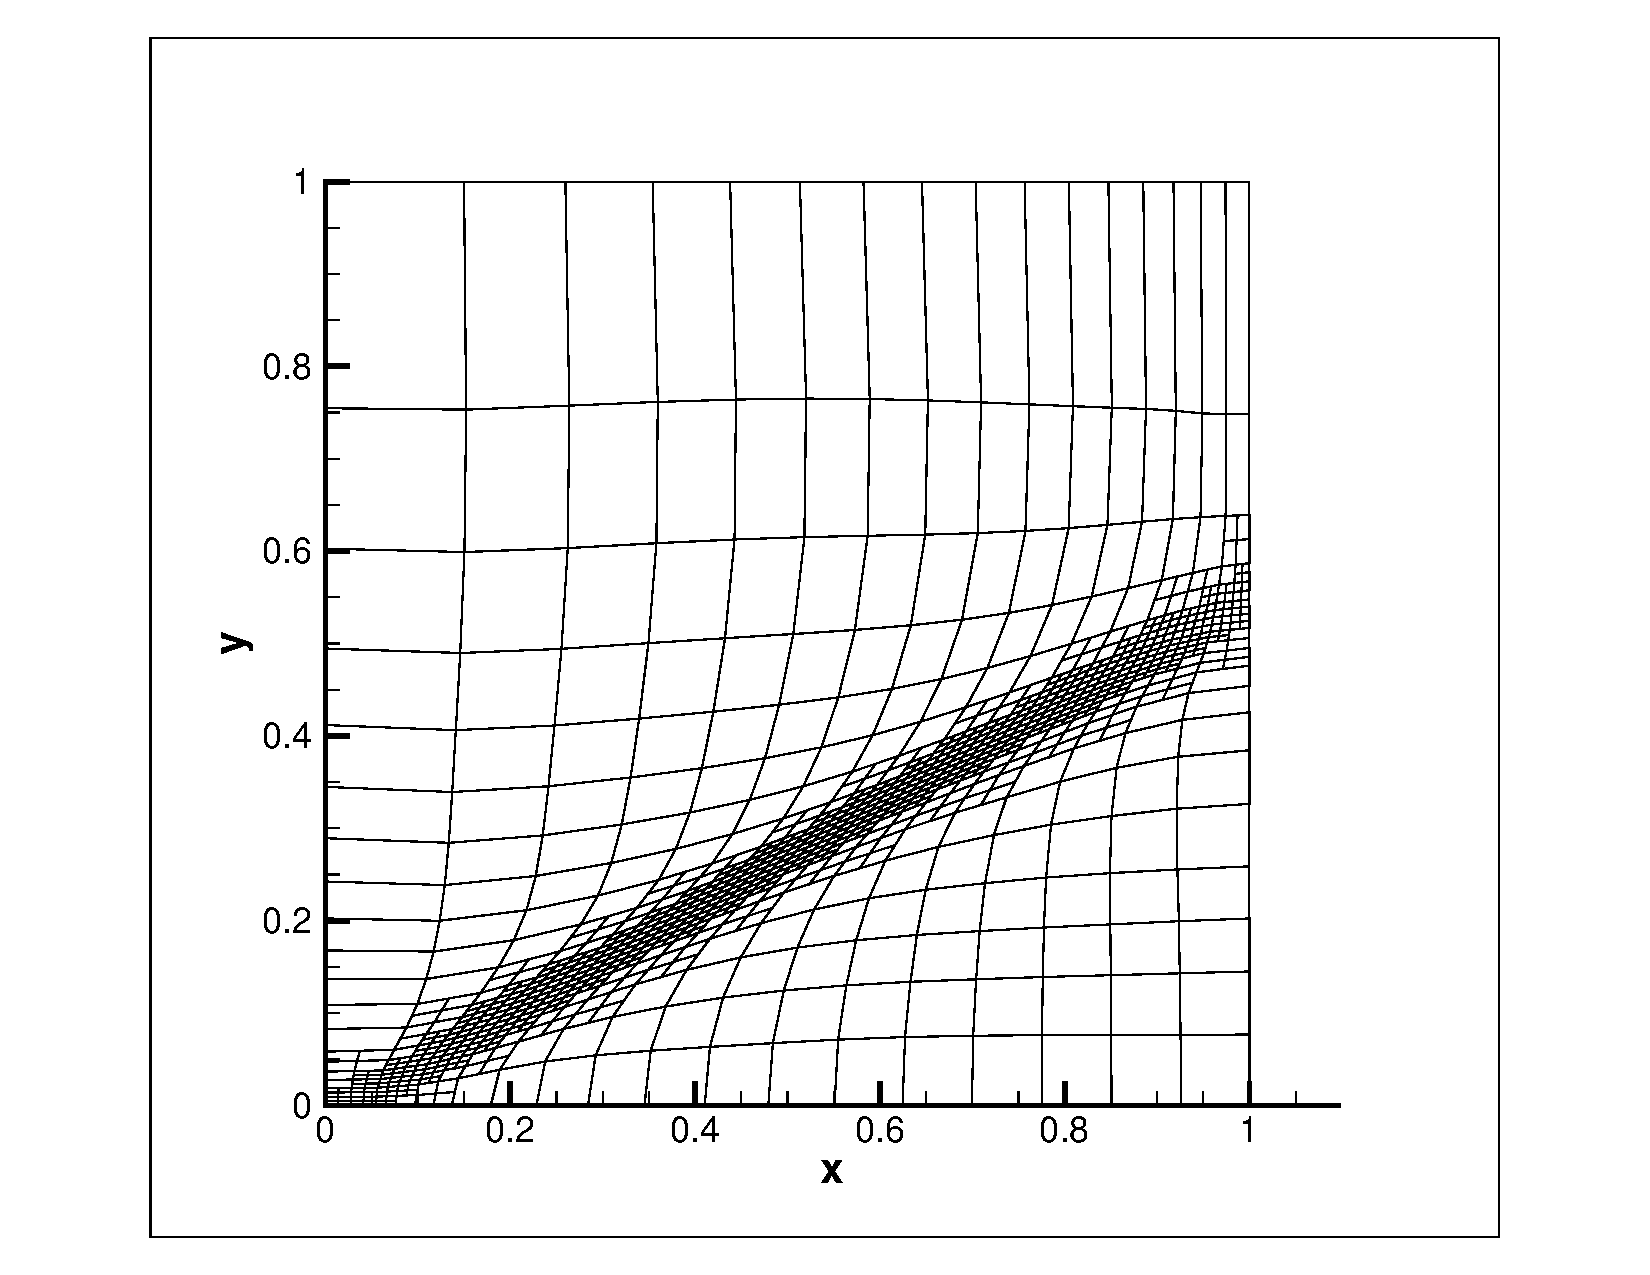
\includegraphics[viewport=110 30 600 550,clip=true,width=.42\textwidth]{fob_redist_adapt_10_mesh.pdf}}
          \subfigure[Solution]{\label{fig:fob_redist_adapt_10_sol}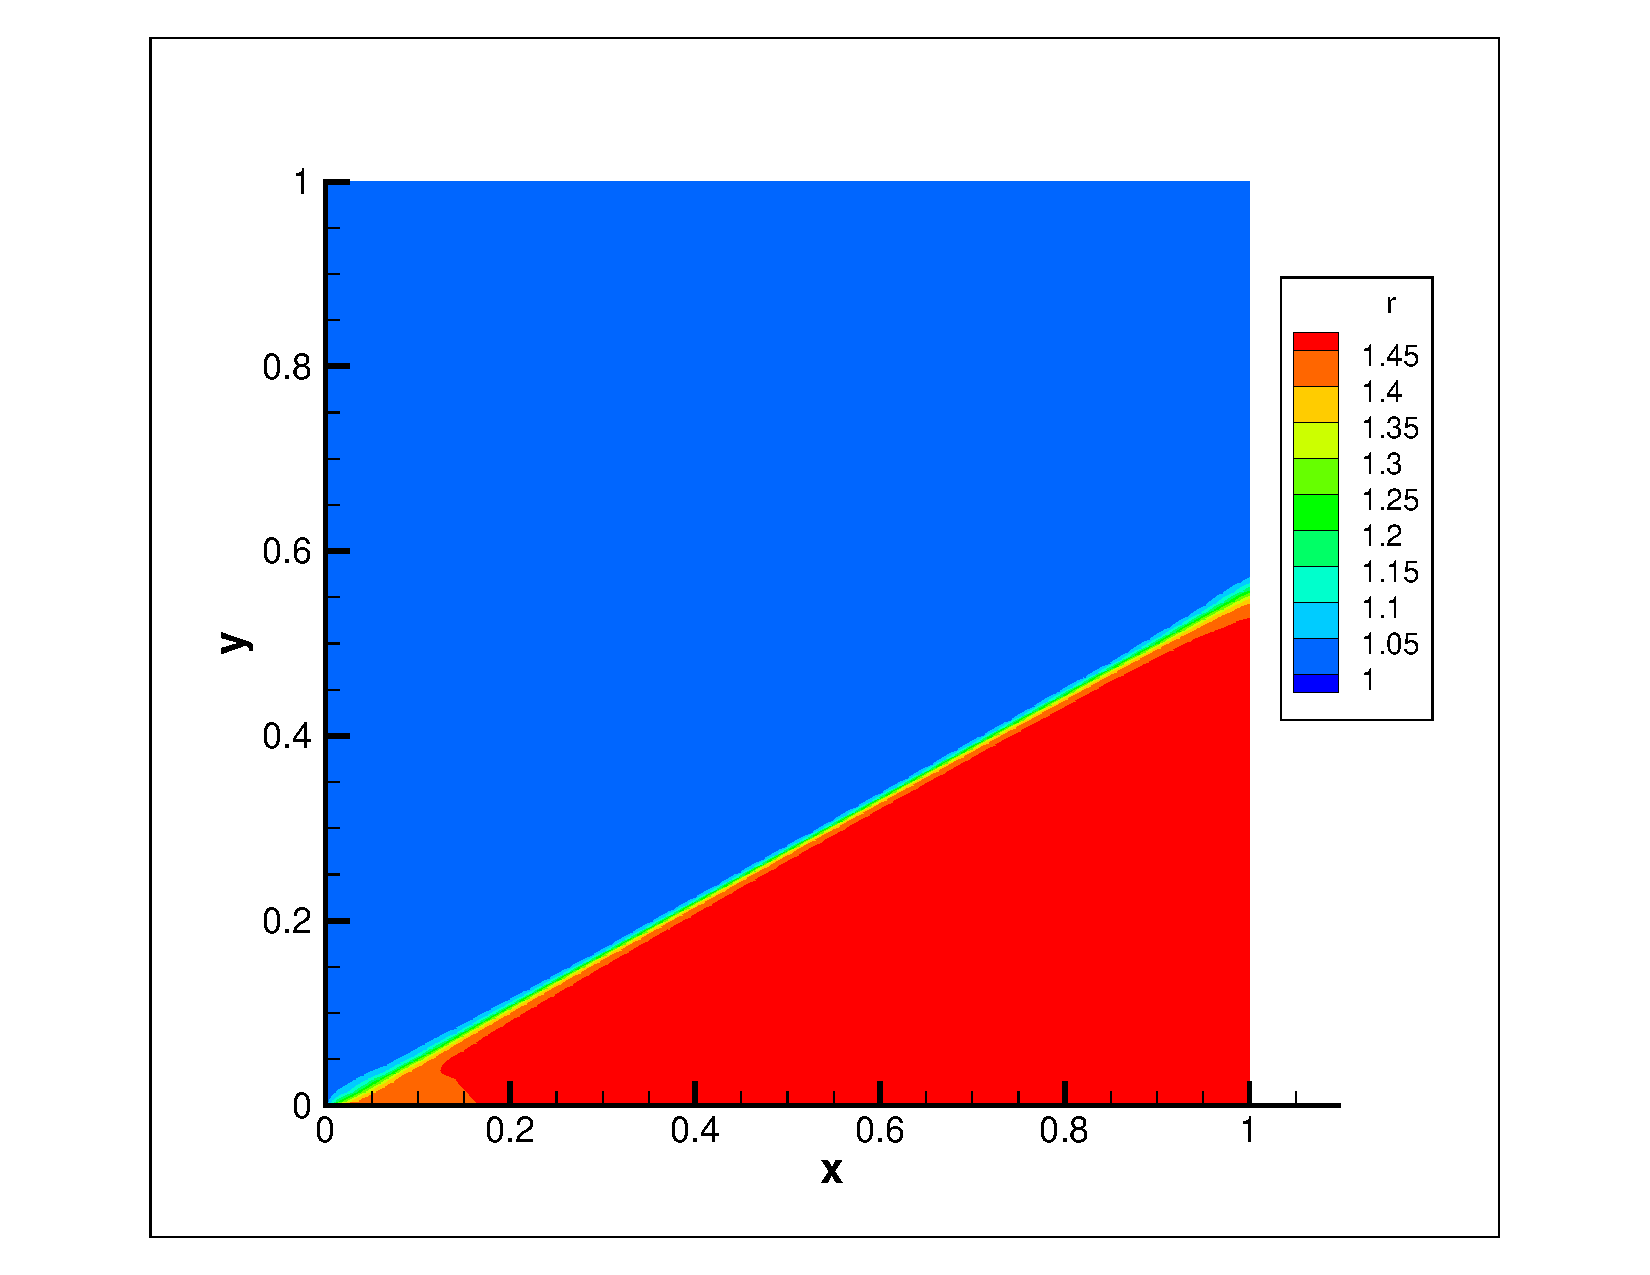
\includegraphics[viewport=110 30 600 520,clip=true,width=.42\textwidth]{fob_redist_adapt_10_sol.pdf}}
        \end{center}
      \end{figure}
  \end{itemize}
}

\frame
{
  \frametitle{Solution Comparison}
  \begin{itemize}[<+->]
    \item For a better comparison here are 3 of the solutions, each with around 11000 DOFs:
      \begin{figure}[!htb]
        \begin{center}
          \subfigure[Uniform.]{\label{fig:fob_uniform_2_sol}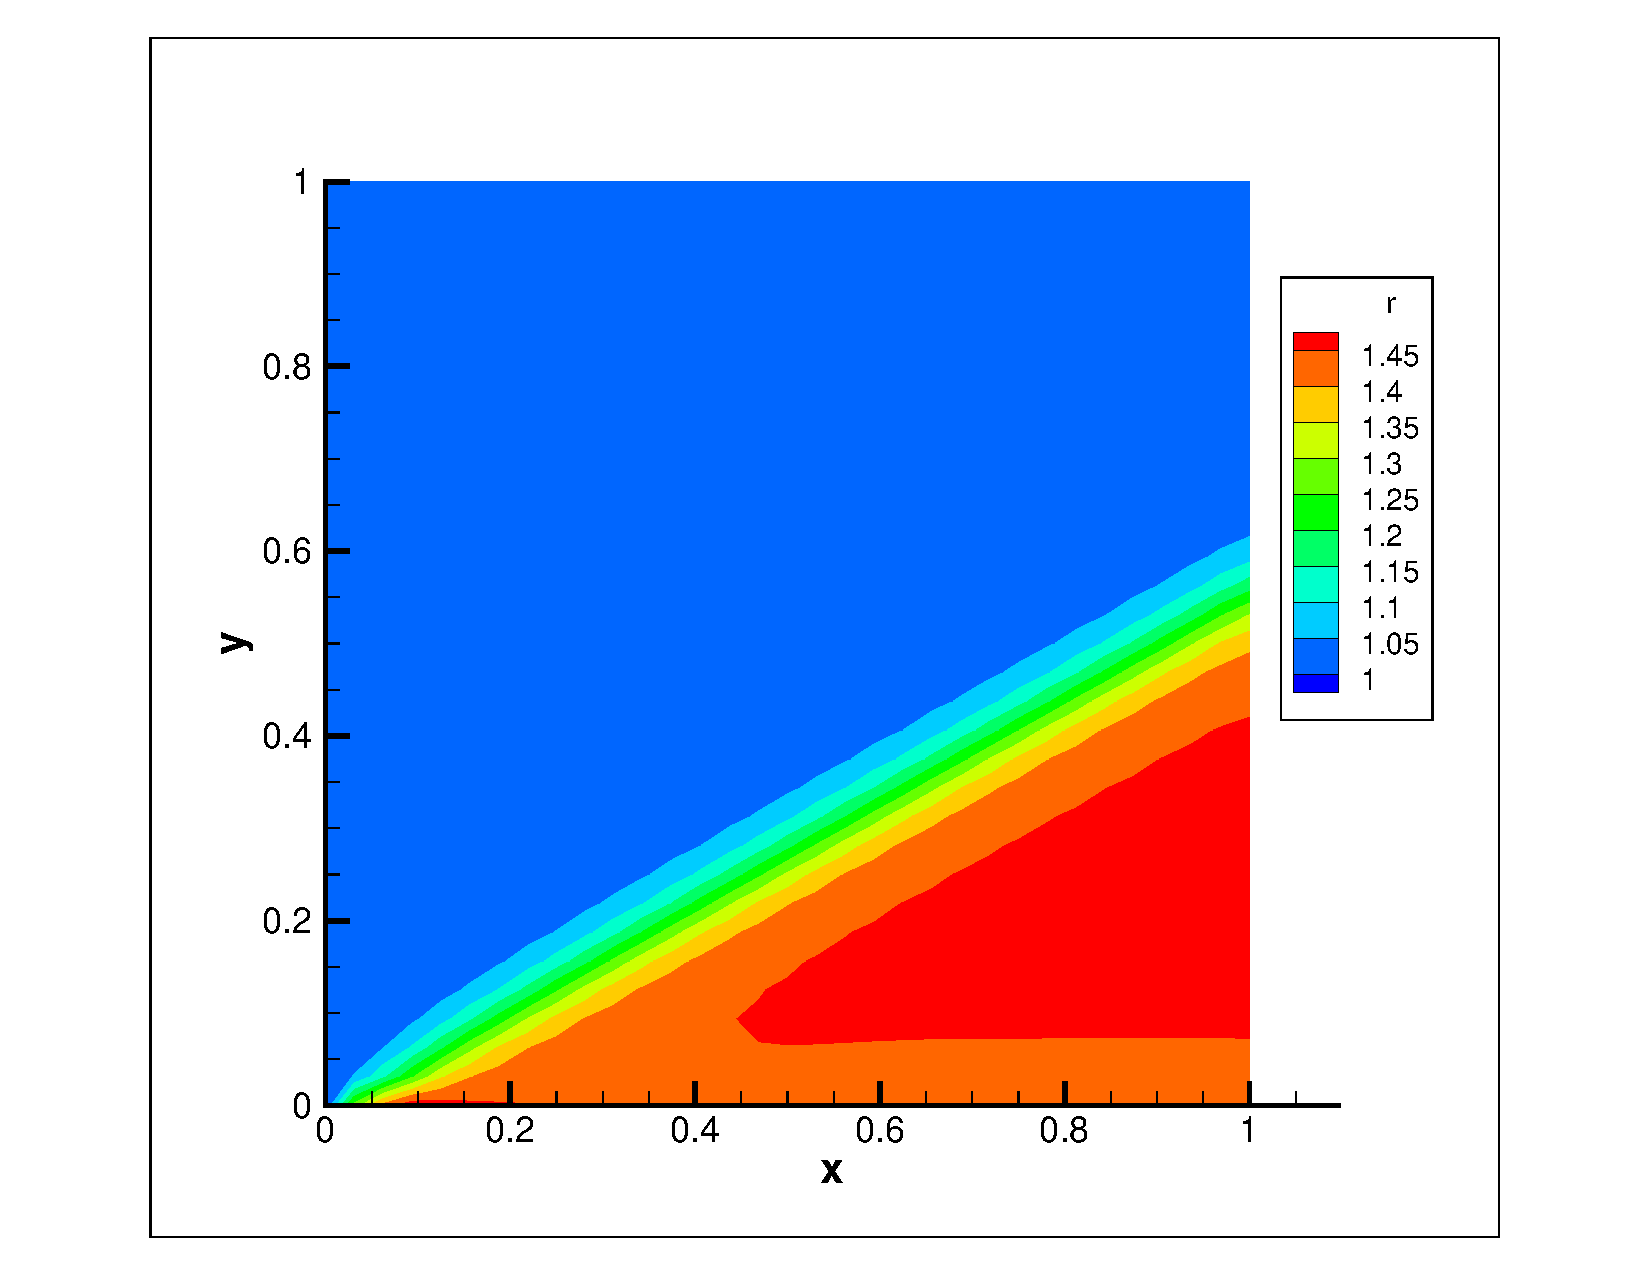
\includegraphics[viewport=110 30 600 520,clip=true,width=.3\textwidth]{fob_uniform_2_sol.pdf}}
          \subfigure[Adaptive.]{\label{fig:fob_adapt_3_sol}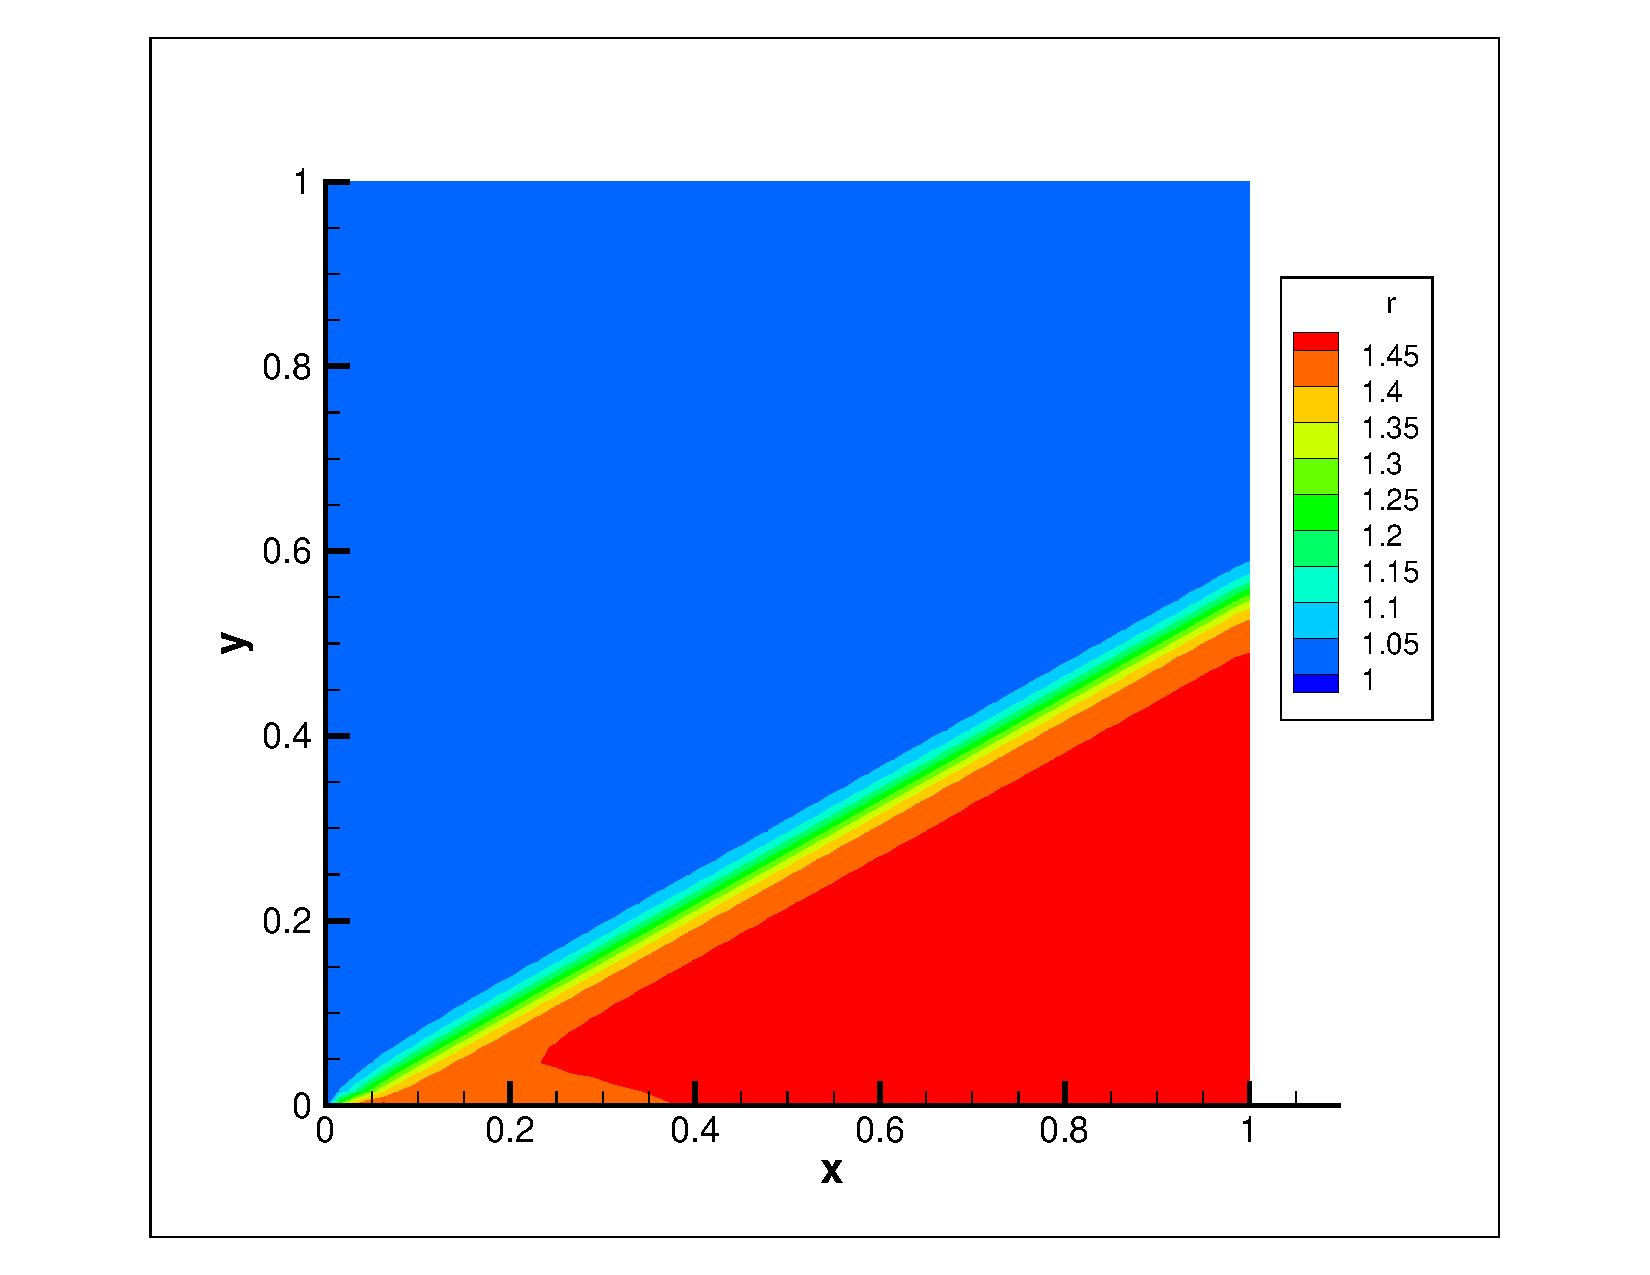
\includegraphics[viewport=110 30 600 520,clip=true,width=.3\textwidth]{fob_adapt_3_sol.pdf}}
          \subfigure[R + H.]{\label{fig:fob_redist_adapt_10_sol}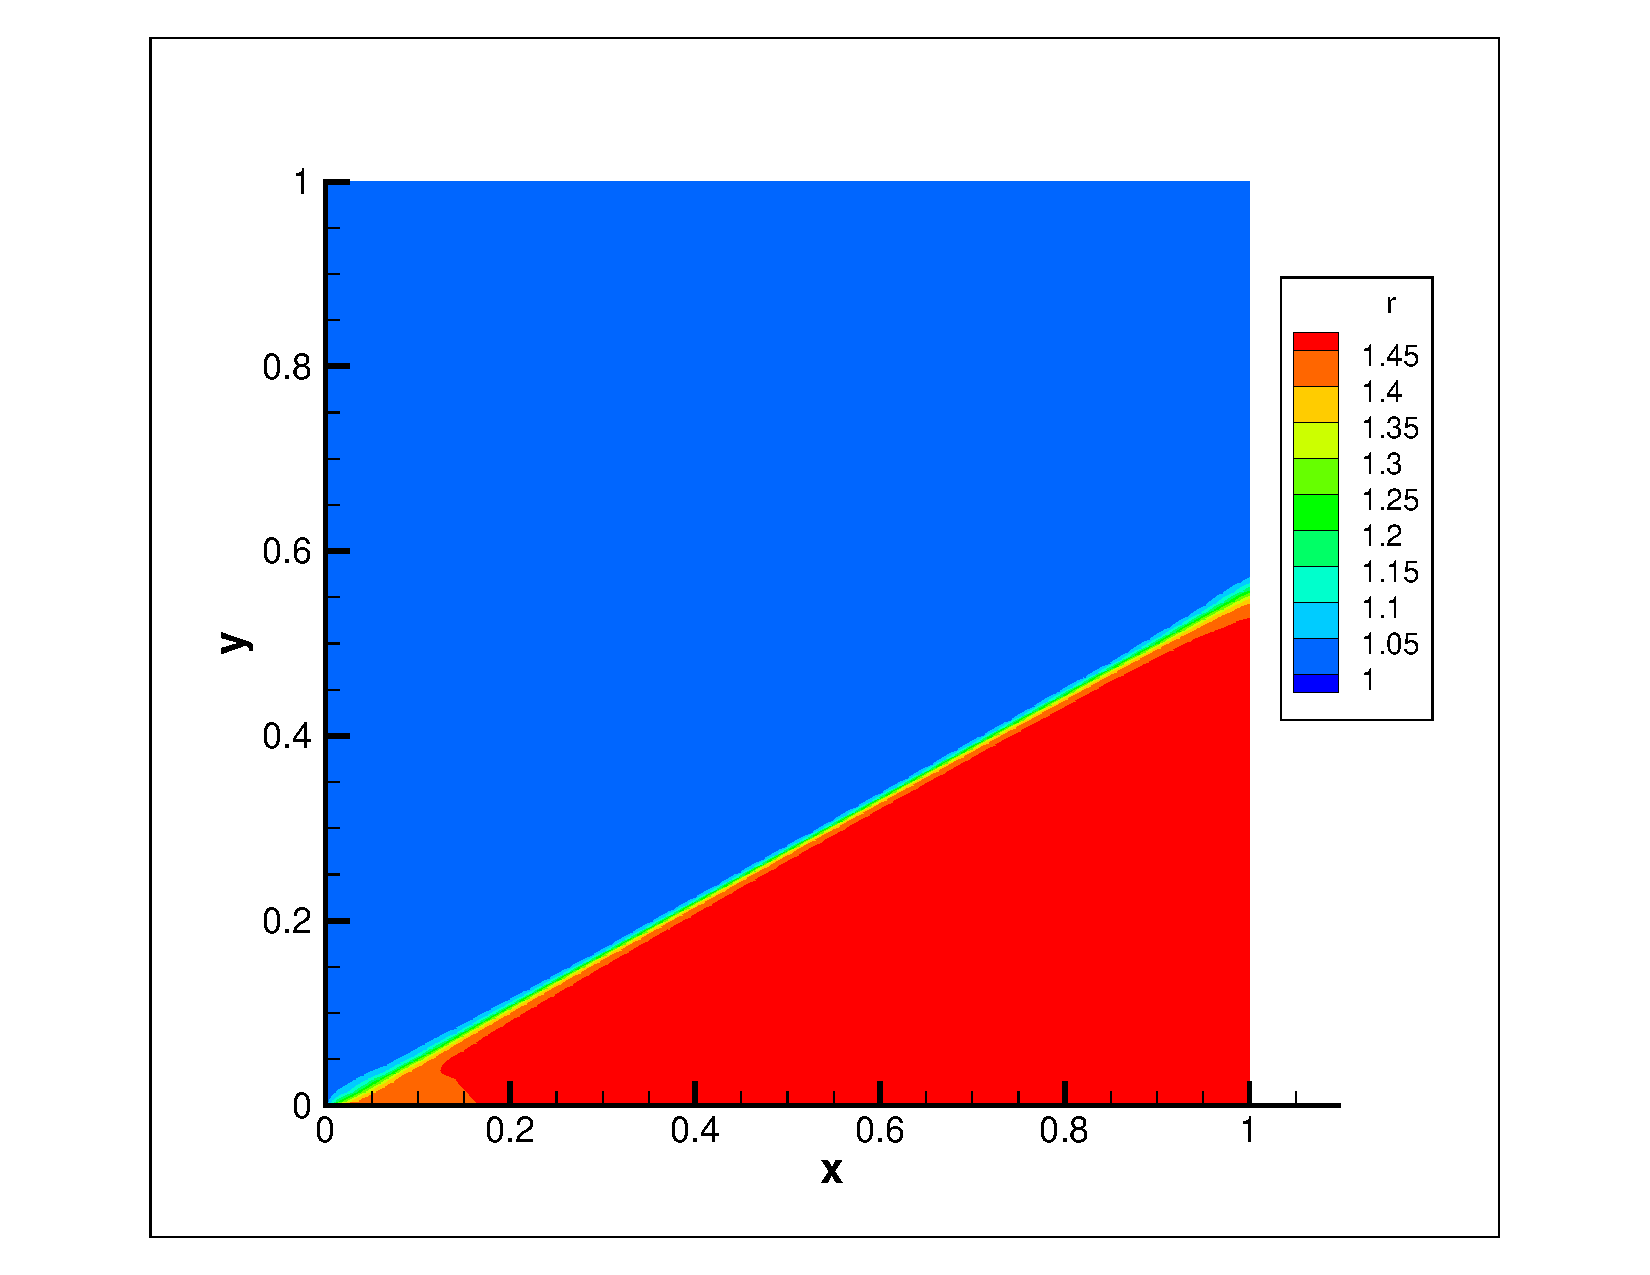
\includegraphics[viewport=110 30 600 520,clip=true,width=.3\textwidth]{fob_redist_adapt_10_sol.pdf}}
        \end{center}
      \end{figure}
  \end{itemize}
}

\frame
{
  \frametitle{Error Plot}
  \begin{itemize}[<+->]
    \item libmesh provides capability for computing error norms against an exact solution.
    \item The exact solution is not in $H^1$ therefore we only obtain
the $L_2$ convergence plot:
      \begin{figure}[!htb]
      \begin{center}
        \subfigure[LogLog plot of L2 vs DOFs.]{\label{fig:fob_l2}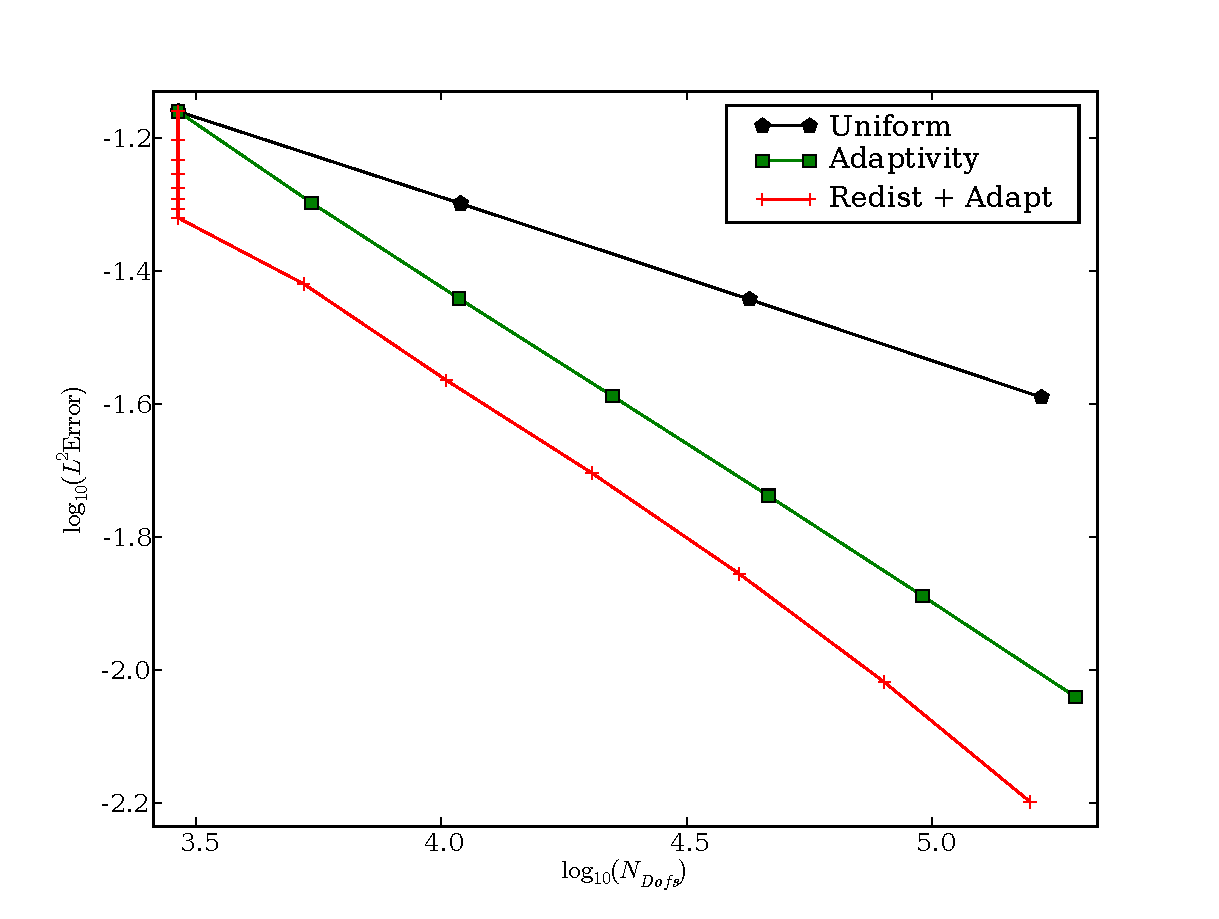
\includegraphics[viewport=0 10 600 400,clip=true,width=.7\textwidth]{fob_l2.pdf}}
      \end{center}
      \end{figure}
  \end{itemize}
}

\frame
{
  %\frametitle{Other Compressible Flow Examples}
    \begin{figure}[!htb]
      \begin{center}
        \subfigure{\label{fig:fob_uniform_2_sol}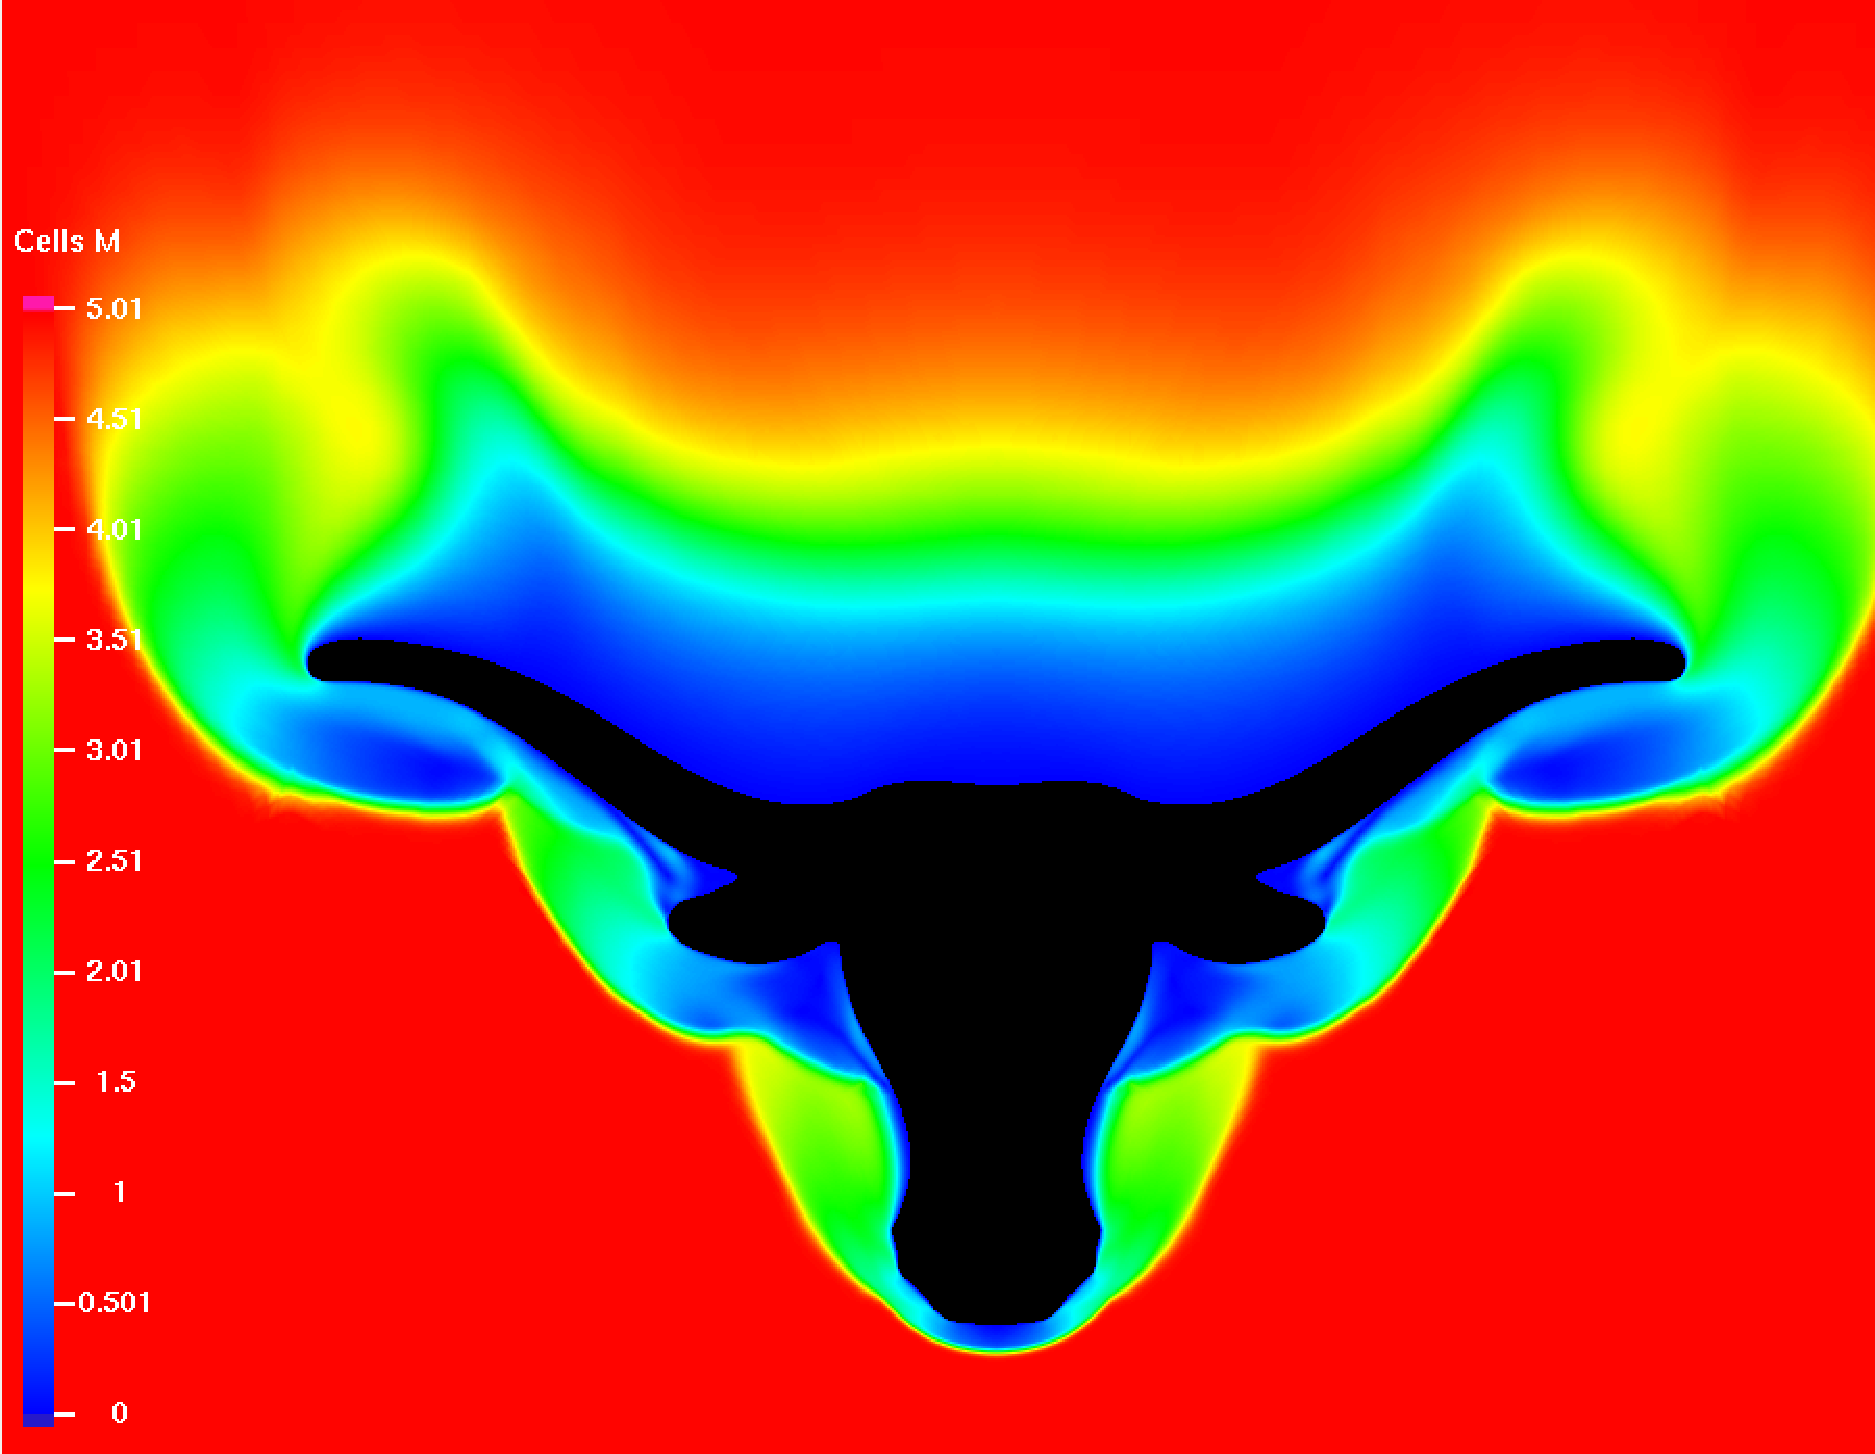
\includegraphics[width=.4\textwidth]{Hypersonic_cow_mach}}
        \subfigure{\label{fig:fob_adapt_3_sol}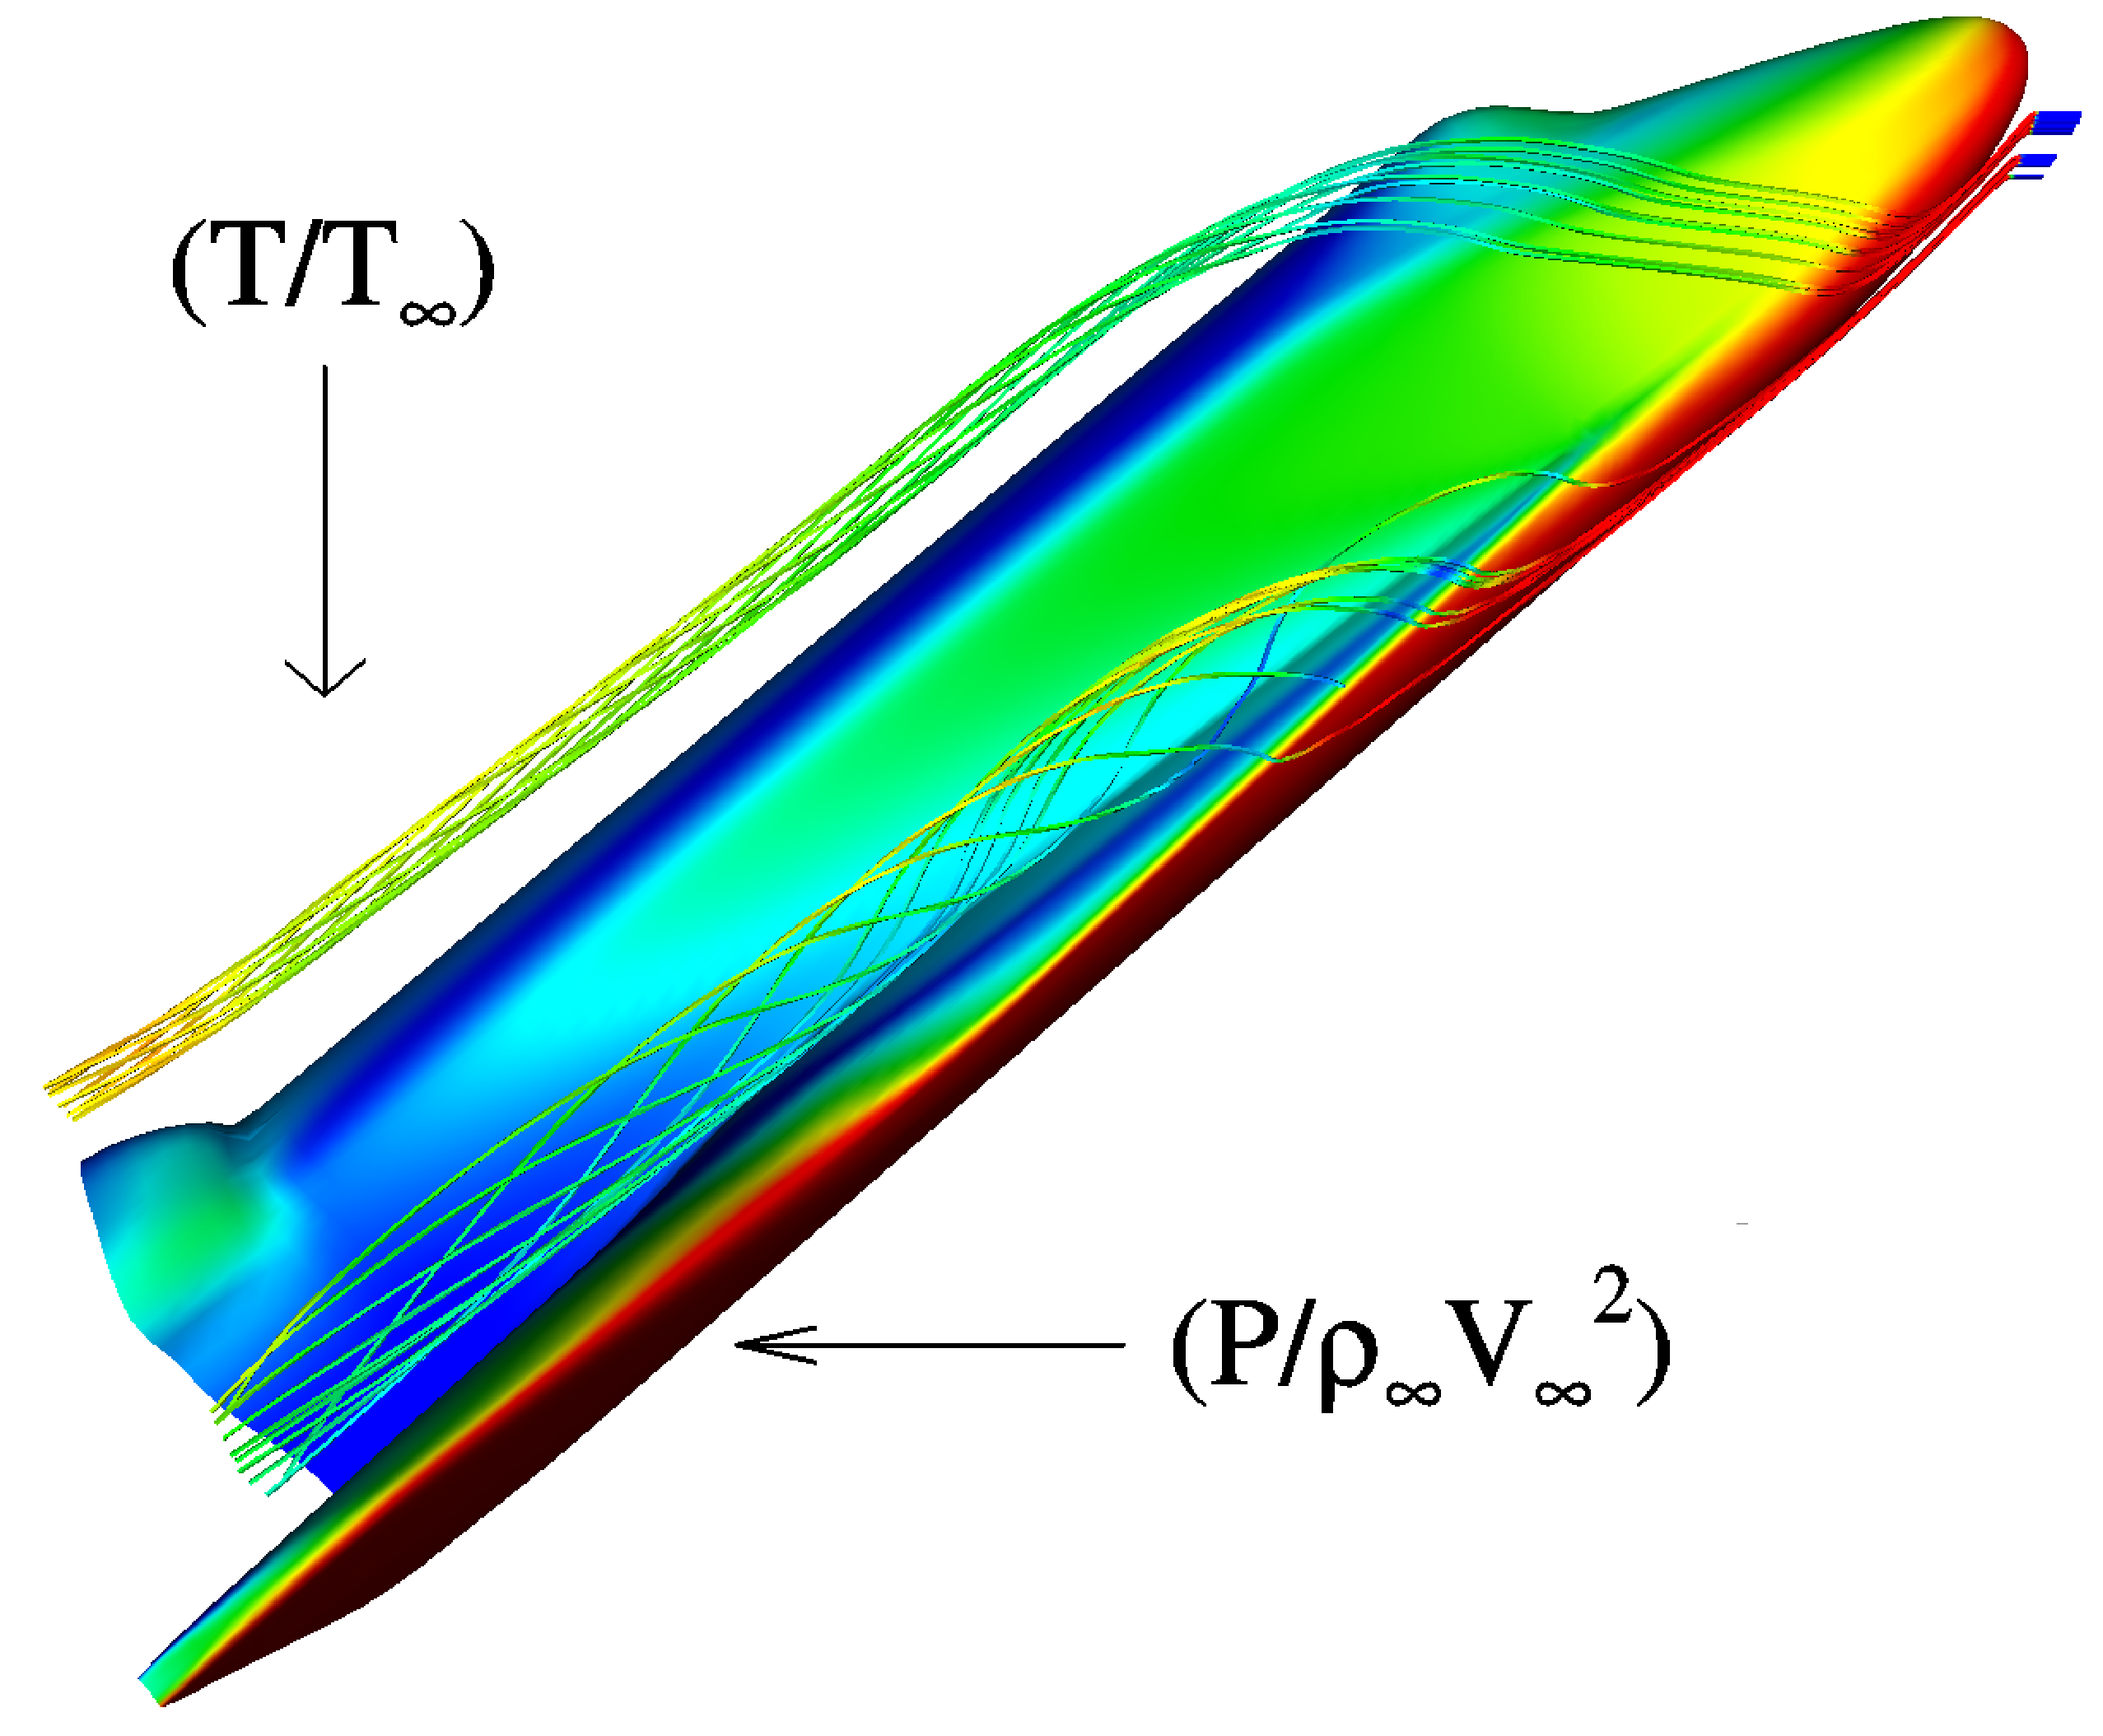
\includegraphics[width=.4\textwidth]{Benkirk_orbiter_reentry_side_view}}
        \subfigure{\label{fig:fob_redist_adapt_10_sol}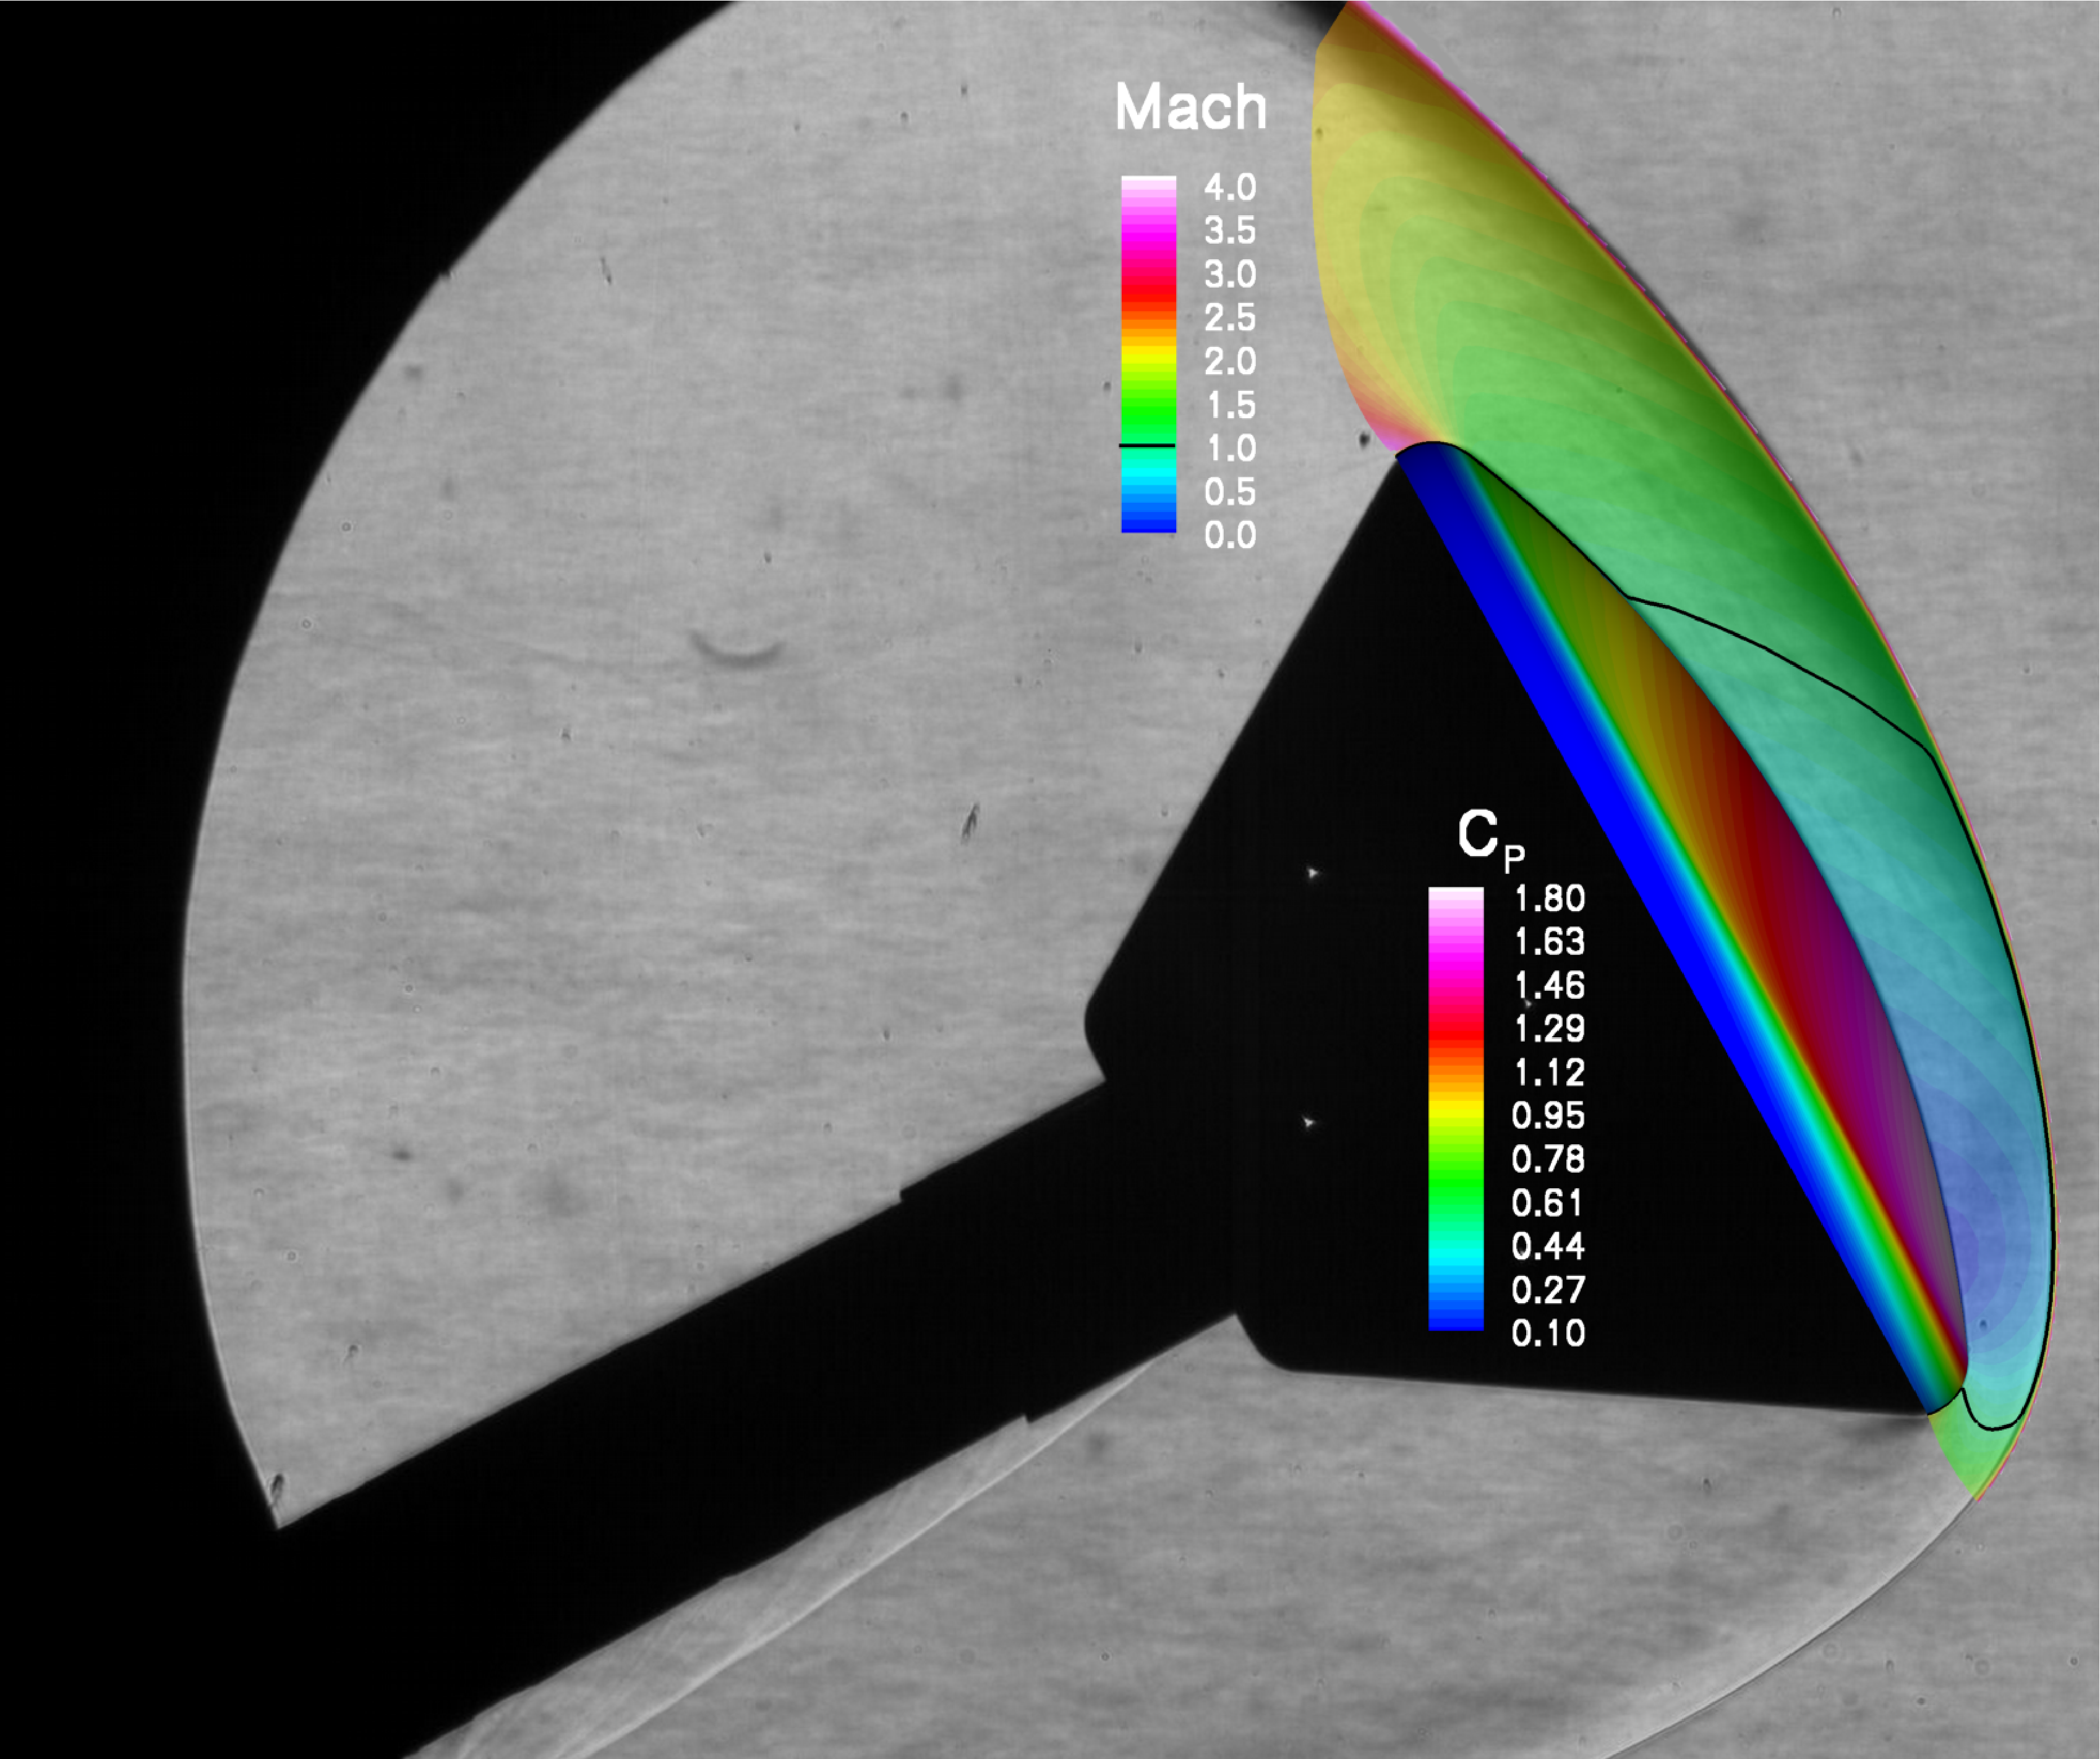
\includegraphics[width=.4\textwidth]{Benkirk_schlieren}}
        \subfigure{\label{fig:fob_redist_adapt_10_sol}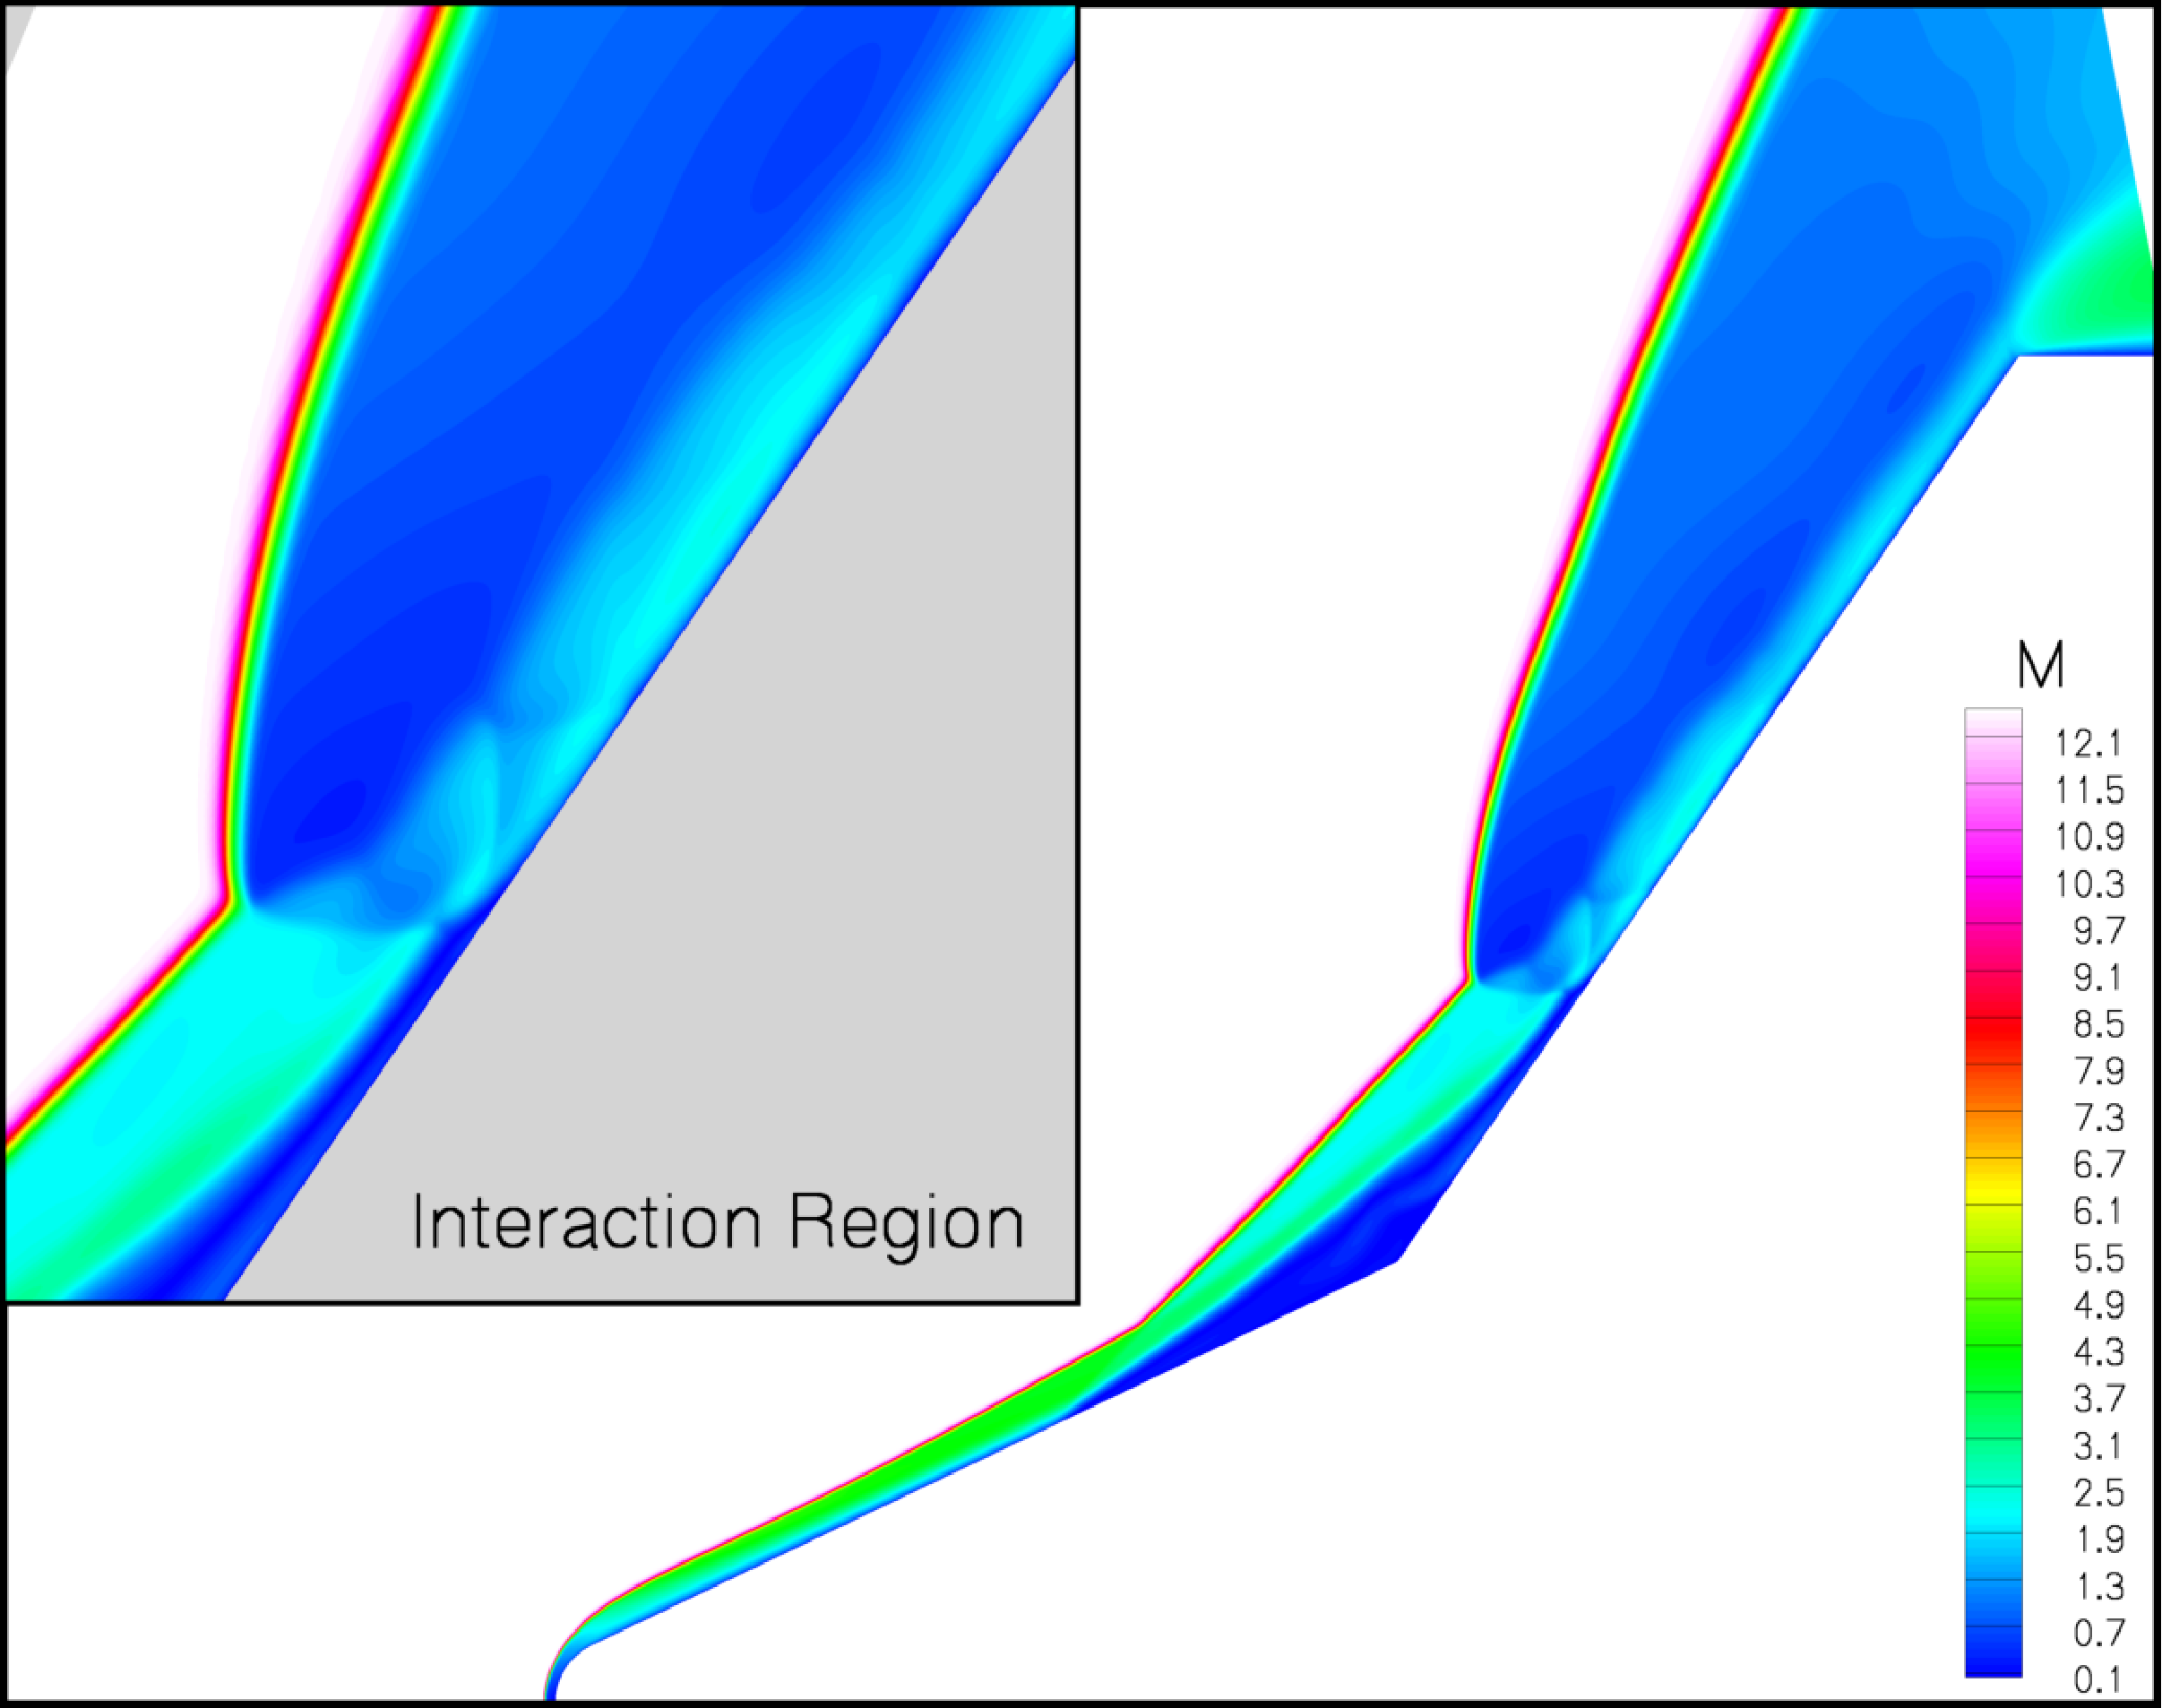
\includegraphics[width=.4\textwidth]{Benkirk_double_cone_M}}
      \end{center}
    \end{figure}
}
